\chapter{Theory}\label{cha:theory}

This chapter introduces the theoretical background on which this analysis is based on.
First, the Standard Model (SM) of particle physics, which describes the fundamental particles and their interactions, is discussed.
Then, an overview of the phenomenology of hadron scattering is given.
Afterwards the Higgs-boson production and decay is discussed in detail and past measurements of the Higgs boson are presented.

\section{The Standard Model of Particle Physics}\label{sec:theory:sm}

The Standard Model of particle physics was developed during the 1960s and 1970s and
describes elementary particles and their fundamental interactions to great precision.
It is a relativistic quantum field theory based on the principle of local gauge symmetries.
Several particles like the $W^\pm$- and $Z^0$- bosons and the top-quark were predicted by the SM and later discovered in
nature~\cite{ZDiscovery,WDiscovery,TopDiscovery,ZeeDiscovery,WeDiscovery,TopDiscoveryD0}.
Out of the four fundamental forces it describes only three, since it was not yet successful to give a
formulation of gravity as a quantum field theory.
But because gravity has only a minor effect on particles at the energy scales accessible at current collider experiments
it can be neglected.

The contents of this section are based on~\cite{Griffiths,HalsenMartin,PeskinSchroeder} if not noted otherwise.

\subsection{Elementary Particles}\label{sub:theory:sm:particles}

The elementary particles of the SM can be divided into fermions which carry half integer spin and bosons with a full integer spin.
Fermions can further be split into leptons which only interact via the electroweak force and quarks which interact via
both the electroweak and strong force.
Empirical evidence shows that there are three generations of both leptons and quarks.
This cannot be predicted by the SM, it was rather used as input.
The three generations are copies of each other which are identical expect for the flavour and mass of the particles.
They are sorted in ascending order by the masses of the particles.
There exist two elementary particles for each generation.

In the case of leptons there is the electron ($e$), muon ($\mu$), and tau lepton ($\tau$) which all have a electric
charge\footnote{The electric charge is given in units of the fundamental electric charge $q_e = \SI{1.602e-19}{\coulomb}$~\cite{PDG}.} of $Q = -1$.
Each lepton is associated with a neutral particle called the neutrino ($\nu_e$, $\nu_\mu$, $\nu_\tau$).

For quarks one particle of each flavour has a electric charge of $Q = \frac{2}{3}$. These particles are called the up-, charm-, and
top-quark.
The other quarks are the down-, strange-, and bottom-quark with charge of $Q = -\frac{1}{3}$.
An overview of the fermions in the SM with their charges and approximate masses is given in \cref{tab:theory:fermions}.

Each particle has its corresponding anti-particle, which has reversed quantum numbers in properties of charge and magnetic momentum.

The matter surrounding us consists only of fermions from the first generation, namely the up- and down-quark which form protons and neutrons and the electron.
All other particles are only accessible via cosmic radiation or accelerator experiments.

\begin{table}[htpb]
    \centering
    \caption{Overview of the fermions in the Standard Model~\cite{PDG}.}\label{tab:theory:fermions}
    \begin{tabular}{lcclcl}
        \toprule
                                 & Generation               & \multicolumn{2}{l}{Flavour}           & Charge [$q_e$] & Mass [GeV] \\  \midrule
        \multirow{6}{*}{Leptons} & \multirow{2}{*}{\nth{1}} & $e$        & Electron                 & $-1$    & $\approx \num{0.5e-3}$ \\
                                 &                          & $\nu_e$    & Electron neutrino        & $ 0$    & $ < \num{2e-9}$        \\ \cmidrule{2-6}
                                 & \multirow{2}{*}{\nth{2}} & $\mu$      & Muon                     & $-1$    & $\approx \num{106e-3}$ \\
                                 &                          & $\nu_\mu$  & Muon Neutrino            & $ 0$    & $ < \num{0.19e-3}$ \\ \cmidrule{2-6}
                                 & \multirow{2}{*}{\nth{3}} & $\tau$     & $\tau$-lepton            & $-1$    & $\approx \num{1.777}$ \\
                                 &                          & $\nu_\tau$ & $\tau$-lepton neutrino   & $ 0$    & $ < \num{18e-3}$ \\ \midrule
        \multirow{6}{*}{Quarks}  & \multirow{2}{*}{\nth{1}} & $u$        & Up                       & $ \frac{2}{3}$ & $\approx \num{2.2e-3}$ \\
                                 &                          & $d$        & Down                     & $-\frac{1}{3}$ & $\approx \num{4.7e-3}$ \\ \cmidrule{2-6}
                                 & \multirow{2}{*}{\nth{2}} & $c$        & Charm                    & $ \frac{2}{3}$ & $\approx \num{1.28}$ \\
                                 &                          & $s$        & Strange                  & $-\frac{1}{3}$ & $\approx \num{96e-3}$ \\ \cmidrule{2-6}
                                 & \multirow{2}{*}{\nth{3}} & $t$        & Top                      & $ \frac{2}{3}$ & $\approx \num{173}$ \\
                                 &                          & $b$        & Bottom                   & $-\frac{1}{3}$ & $\approx \num{4.18}$ \\
        \bottomrule
    \end{tabular}
\end{table}

The fundamental interactions of the SM are mediated by gauge bosons with spin one.
An overview of the gauge bosons in the SM is given in \cref{tab:theory:bosons}.

The photon ($\gamma$) is the mediator of the electromagnetic force.
It couples to the electric charge $Q$ of the particles.
Due to the fact that the photon is massless, the electromagnetic force has infinite range.

The weak interaction is transmitted via the massive $W^\pm/Z^0$-bosons, which couple to the weak isospin $I_w$ of the particles.
All fermions have a weak isospin of $I_w = \frac{1}{2}$ and the bosons of  $I_w = 1$.
In contract to the photon the $W^\pm$- and $Z^0$-bosons are quite massive with a mass of $m_{W^\pm} = \SI{80.4}{\GeV}$ and
$m_{Z^0} = \SI{91.2}{\GeV}$, respectively~\cite{PDG}.
This leads to the weak coupling at low energies and the low range of the weak interaction.
Additionally, the $W^\pm/Z^0$-bosons can interact with themselves.

The strong force is mediated by eight gluons ($g$), which are massless and couple to the color charge.
All quarks and gluons have a color charge.
Because the gluons have a color charge themselves, self-interaction is possible, which limits the range of the
strong force.

\begin{table}[htpb]
    \centering
    \caption{Overview of the gauge bosons in the Standard Model~\cite{PDG}.}\label{tab:theory:bosons}
    \begin{tabular}{lclccc}
        \toprule
        Interaction             & \multicolumn{2}{l}{Gauge boson}   & Charge [$q_e$]    & Mass [GeV] & Range [m] \\  \midrule
        Electromagnetic         & $\gamma$  & Photon                & $0$               & 0          & $\infty$                         \\ \cmidrule{1-6}
        \multirow{2}{*}{Weak}   & $W^\pm$   & $W^\pm$ boson         & $\pm 1$           & 80.4       & \multirow{2}{*}{$< \num{e-15}$}  \\
                                & $Z^0$     & $Z^0$ boson           & $0$               & 91.2       &                                  \\ \cmidrule{1-6}
        Strong                  & $g$       & Gluon (8x)            & $0$               & 0          & $\approx \num{e-15}$             \\
        \bottomrule
    \end{tabular}
\end{table}

The Standard Model contains also one scalar spin-0 particle, the Higgs boson.
It has been detected in 2012 with the ATLAS and CMS detectors~\cite{HiggsDiscoveryATLAS,HiggsDiscoveryCMS}.
The Higgs boson has a mass of $m_H = \SI{125}{\GeV}$~\cite{MassCombinedMeas}, no electric or color charge, a weak isospin of $I_w = \frac{1}{2}$, and a
weak hypercharge of $Y = 1$.
The Higgs boson and the current measurements of Higgs-boson properties are discussed in detail in \cref{sec:theory:higgs,sec:theory:measurements}.

\subsection{Fundamental interactions}\label{sub:theory:sm:interactions}

A gauge theory is a field theory where the Lagrangian density is invariant under a group of global or local transformations.
In the Standard Model the fundamental interactions are described by local gauge symmetries.
The symmetries force a certain structure on the Lagrangian, which reflects in the resulting theory.
The correct symmetry group has to be selected based on empirical observations, so that theory predictions are in agreement with measurements.

\subsubsection{Quantum Electrodynamics}

The electromagnetic interaction is described by Quantum Electrodynamics (QED), which is based on the $U(1)_Q$ symmetry group.
It is carried by the photon, which is massless and couples to the electric charge $Q$.
A free fermion with mass $m$ can be described by the Lagrangian density
\begin{equation}
    \label{eq:theory:qed:l}
    \lagl = \psibar \left( i \gamma^\mu \partial_\mu - m\right) \psi \,,
\end{equation}
where the Dirac spinor is denoted as $\psi$, the gamma matrices as $\gamma^\mu$, and the partial derivative as $\partial_\mu = \frac{\partial}{\partial x^\mu}$.
By applying the Euler--Lagrange equation,
\begin{equation}
    \frac{\partial \lagl}{\partial \psibar} - \partial^\mu \left( \frac{\partial \lagl}{\partial \left(\partial^\mu \psibar \right)} \right) = 0 \,,
\end{equation}
the corresponding equation of motion can be obtained,
\begin{equation}
     \left( i \gamma^\mu \partial_\mu - m\right) \psi = 0\,.
\end{equation}
Because every gauge theory is required to be invariant under local transformations of the symmetry group, the lagrangian density in \cref{eq:theory:qed:l} has to be
invariant under local transformations of the $U(1)_Q$ group, which have the following form:
\begin{equation}
    \psi \mapsto \psi' = e^{-iQ\alpha(x)} \psi \,.
\end{equation}
The operator of electric charge is denoted as $Q$ and the local phase depending on time and space as $\alpha(x)$.
However, if this transformation is applied to \cref{eq:theory:qed:l} an additional term appears and the
gauge invariance is broken,
\begin{equation}
    \partial_\mu \psi \mapsto \partial_\mu \psi' = -i Q \alpha(x) \psi + e^{-iQ\alpha(x)} \partial_\mu \psi \,.
\end{equation}
To restore the gauge invariance a new vector field $A_\mu$, which transforms as
\begin{equation}
    A_\mu \mapsto A'_\mu = A_\mu + \partial_\mu \alpha(x) \,,
\end{equation}
and the covariant derivative,
\begin{equation}
    D_\mu = \partial_\mu + i q A_\mu \,,
\end{equation}
need to be introduced.
The gauge-invariant Lagrangian density of QED reads
\begin{equation}
    \lagl = \psibar \left( i \gamma^\mu D_\mu -m \right) \psi \,.
\end{equation}
The new vector field $A_\mu$ couples to fermions with a coupling strength of $Q_f$ and ensure the local gauge invariance.
It can be identified with the photon when a kinematic term, which is formed by the field strength tensor
\begin{equation}
    F_{\mu \nu} = \partial_\mu A_\nu - \partial_\nu A_\mu \,,
\end{equation}
is added to the Lagrangian density,
\begin{equation}
    \lagl_\text{QED} = \psibar \left( i \gamma^\mu D_\mu -m \right) \psi - \frac{1}{4} F^{\mu\nu} F_{\nu\nu} \,.
\end{equation}
If a mass term of the form $-\frac{1}{2}m^2 A^\mu A_\mu $ was introduced, it would break gauge invariance again.
Therefore, a massless photon is required in QED, which corresponds with the upper limit of the photon mass of $m_\gamma < \SI{3e-27}{\eV}$
obtained by experimental measurements~\cite{PhotonMass}.

\subsubsection{Quantum Chromodynamics}

The interaction of quarks and gluons via the strong force is described by Quantum Chromodynamics (QCD), which is based on the $SU(3)_C$ symmetry group.
The charge associated with the strong interaction is the color charge, which is the equivalent to the electric charge in QED\@.
Experimental measurements show that there are three different color states: red, green, and blue.
Those three states can be described by building a vector of three spinor fields, which replaces the single Dirac spinor $\psi$ from QED,
\begin{equation}
    \psi =
    \begin{pmatrix}
        \psi_\text{red} \\
        \psi_\text{green} \\
        \psi_\text{blue} \\
    \end{pmatrix} \,.
\end{equation}
Under a local $SU(3)_C$ transformation a free quark field $\psi(x)$ transforms like
\begin{equation}
    \psi(x) \mapsto \psi'(x) = \exp \left[ i \frac{g_s}{2} \sum_{a=1}^8 \lambda_a \beta_a (x) \right] \psi(x) \,.
\end{equation}
Here, the coupling strength is denoted as $\alpha_s$, the eight Gell-Mann matrices as $\lambda_a$, and the $\beta$ functions of QCD as $\vec{\beta}(x)$~\cite{Schmuser}.
In the following the gauge coupling parameter $g_s = \sqrt{4 \pi \alpha_s}$ is used instead of the coupling strength.

The $SU(3)_C$ group is a \emph{non-abelian} group, since its generators do not commute.
This results in an additional term in the field strength tensor $G_{\mu\nu}^a$ of the gluon fields $G_\mu^a$ ($a = 1, \ldots, 8$),
\begin{equation}
    G_{\mu\nu}^a = \partial_\mu G_\nu^a -  \partial_\nu G_\mu^a - g_s f^{abc} G_\mu^b G_\nu^c \,,
\end{equation}
with the structure constants $f^{abc}$ of the $SU(3)_C$ group.
Because there are eight Gell-Mann matrices, which are the generators of $SU(3)_C$, there are also eight gluon fields defined.

To ensure gauge invariance again a covariant derivative is introduced,
\begin{equation}
    D_\mu = \partial_\mu + i g_s \frac{\lambda_a}{2} G_\mu^a \,.
\end{equation}
The Lagrangian density of QCD can then be written as
\begin{equation}
    \lagl_\text{QED} = \psibar \left( i \gamma^\mu D_\mu -m \right) \psi - \frac{1}{4} G^{\mu\nu} G_{\nu\nu} \,.
\end{equation}
The non-abelian structure of $SU(3)_C$ leads to gluon self-interaction.
Similarly to photons, the gluons need also to be massless to ensure the gauge invariance, which agrees with experimental observations.
Because of the gluon self-interaction the strong force has not unlimited range.
At very short distances, the strong force becomes weak, which is also known as \emph{asymptotic freedom}~\cite{AsymFreedom1,AsymFreedom2}.
For interactions and long distances the interaction potential increases for color-charged particles.
Therefore, free quarks are not stable but form colorless bound states which are called mesons (quark and anti-quark) and
baryons (three quarks or three anti-quarks).
This is called \emph{confinement}.

For quarks a mass term is allowed and does not break the symmetry, unlike for gluons.
The masses are different for each flavour but do not depend on the color charge.

\subsubsection{Electroweak Interaction}

The weak interaction is mediated by the charged $W^\pm$-bosons and the neutral $Z^0$-boson, which couple to the weak
isospin, $I_w$.
The exchange of a $W^\pm$-boson is called \emph{charged current}, because it modifies the flavour of fermions and causes a change in the electric charge of $\Delta Q = 1$.
In contrast, the exchange of a $Z$-boson does not change the flavour of quarks, which leads to the name \emph{neutral current}.
It was discovered that weak interactions mediated by $W^\pm$-bosons are maximally parity violating, because the bosons couple only to
left-handed particles and right-handed anti-particles~\cite{PhysRev.104.254,PhysRev.105.1413}.
This lead to the combination of the electromagnetic and weak interaction by Glashow, Salam, and Weinberg in the
so-called electroweak Standard Model~\cite{Glashow1961,Salam1959,Weinberg1967}.

The electroweak interaction is based on an underlying $SU{(2)}_{L,I_w} \times U{(1)}_Y$ symmetry
and is able to describe both the electromagnetic and weak interaction.
Here, the hypercharge $Y$ was introduced and $L$ denotes the coupling to only left-handed particles.
A connection between the electric charge $Q$, the hypercharge $Y$, and the third component of the weak isospin $I_3$
is given by the Gell-Mann--Nishijima formula~\cite{Nishijima1955,GellMann1956},
\begin{equation}
    Q = I_3 + \frac{Y}{2} \,.
\end{equation}
Left-handed fermions are described by $SU{(2)}_{L,I_w}$ doublets with $I_w = \frac{1}{2}$ and $I_3 = \pm \frac{1}{2}$.
Right-handed fermions are assigned to $SU{(2)}_{L,I_w}$ singlets with $I_w = I_3 = 0$.
An overview of the quantum numbers of fermions in the electroweak theory is given in \cref{tab:theory:quantumnumbers}.
Right-handed neutrinos are not included, since they do not couple to other particles of the SM\@.
Recent results from neutrino-oscillation experiments which also yielded a Nobel Price in Physics in 2015 show that at
least two neutrino masses are not zero~\cite{NeutrinoOsc1,NeutrinoOsc2,NeutrinoOsc3,NeutrinoOsc4,NeutrinoOsc5,NeutrinoOsc6}.
However, in this thesis neutrinos are assumed to be massless.

Quarks are described in weak eigenstates ($d',s',b'$) with $I_3 = -\frac{1}{2}$ which are a mixture of their mass eigenstates ($u, s, b$).
The degree of mixing is described by the Cabibbo--Kobayashi--Maskawa (CKM) matrix~\cite{CKM:KM,CKM:C},
\begin{equation}
    \begin{pmatrix}
        d' \\ s' \\ b' \\
    \end{pmatrix}
    =
    \begin{pmatrix}
        V_{ud} & V_{us} & V_{ub} \\
        V_{cd} & V_{cs} & V_{cb} \\
        V_{td} & V_{ts} & V_{tb} \\
    \end{pmatrix}
    \begin{pmatrix}
        d \\ s \\ b \\
    \end{pmatrix} \,.
\end{equation}
The elements $\abs{V_{ij}}^2$ give the probability of a quark changing its flavour from $i$ to $j$ when interacting with a $W^\pm$-boson.
Due to the non-vanishing complex phase of the CKM matrix the CP invariance is violated~\cite{PhysRevLett.13.138}.

\begin{table}[tb]
    \centering
    \caption{Overview of singlets and doublets in the electroweak theory and their associated quantum numbers.}\label{tab:theory:quantumnumbers}
    \begin{tabular}{cccccccc}
        \toprule
         & \multicolumn{3}{c}{Generations} & \multicolumn{4}{c}{Quantum numbers} \\ \cmidrule{2-8}
         & \nth{1} & \nth{2} & \nth{3} & $I_w$ & $I_3$ & $Y$ & $Q$ [$q_e$] \\ \midrule
        \multirow{3}{*}{Leptons} & \multirow{2}{*}{${\begin{pmatrix}\nu_e \\ e \end{pmatrix}}_L$}
                                 & \multirow{2}{*}{${\begin{pmatrix}\nu_\mu \\ \mu \end{pmatrix}}_L$}
                                 & \multirow{2}{*}{${\begin{pmatrix}\nu_\tau \\ \tau \end{pmatrix}}_L$} & $\frac{1}{2}$ & $\frac{1}{2}$ & $-1$ & $0$ \\
         & & & & $\frac{1}{2}$ & $-\frac{1}{2}$ & $-1$ & $-1$ \\
         & $e_R$ & $\mu_R$ & $\tau_R$ & $0$ & $0$ & $-2$ & $-1$ \\ \cmidrule{1-8}
        \multirow{4}{*}{Quarks} & \multirow{2}{*}{${\begin{pmatrix}u \\ d' \end{pmatrix}}_L$}
                                & \multirow{2}{*}{${\begin{pmatrix}c \\ s' \end{pmatrix}}_L$}
                                & \multirow{2}{*}{${\begin{pmatrix}t \\ b' \end{pmatrix}}_L$} & $\frac{1}{2}$ & $\frac{1}{2}$ & $\frac{1}{3}$ & $\frac{2}{3}$ \\
         & & & & $\frac{1}{2}$ & $-\frac{1}{2}$ & $\frac{1}{3}$ & $-\frac{1}{3}$ \\
         & $u_R$ & $c_R$ & $t_R$ & $0$ & $0$ & $\frac{4}{3}$ & $\frac{2}{3}$ \\
         & $d_R$ & $s_R$ & $b_R$ & $0$ & $0$ & $-\frac{2}{3}$ & $-\frac{1}{3}$ \\
         \bottomrule
    \end{tabular}
\end{table}

Left-handed isospin doublets transform under the $SU{(2)}_{L,I_w}$ symmetry as
\begin{equation}
    \psi_L(x) \mapsto \psi'_L(x) = \exp \left[ i \frac{g}{2} \sum_{a=1}^{3} \tau_a \alpha_a(x) \right] \psi_L(x) \,,
\end{equation}
with the generators $\tau_a/2$ ($a = 1, 2, 3$) of the $SU{(2)}_{L,I_w}$ symmetry which are the $2\times 2$ Pauli matrices,
the coupling strength $g$, and the local phase $\alpha_a(x)$.
The left-handed isospin doublets and the right-handed singlets transform have the following transformation behavior under the $U{(1)}_Y$ symmetry:
\begin{gather}
    \psi_L(x) \mapsto \psi'_L(x) = \exp \left[ i \frac{g'}{2} Y \beta(x) \right] \psi_L(x) \,, \\
    \psi_R(x) \mapsto \psi'_R(x) = \exp \left[ i \frac{g'}{2} Y \beta(x) \right] \psi_R(x) \,,
\end{gather}
where $g'$ is a second coupling constant, $Y$ the generator of the hypercharge, and $\beta(x)$ the local phase.

To preserve gauge invariance three vector fields $W^a$ ($a = 1,2,3$) for $SU{(2)}_{L,I_w}$ and one gauge field $B$
for $U{(1)}_Y$ need to be introduced.
With the covariant derivatives for left- and right-handed fermion fields,
\begin{align}
    \label{eq:theory:ew:D}
    D_\mu^L &= \partial_\mu + i \frac{g}{2} \tau_a W_\mu^a + i \frac{g'}{2} Y B_\mu \,, \\
    D_\mu^R &= \partial_\mu + i \frac{g'}{2} Y B_\mu \,,
\end{align}
the Lagrangian density for the electroweak interaction reads
\begin{equation}
    \label{eq:theory:ew:l}
    \lagl_\text{EW} = \psibar_L i \gamma^\mu D_\mu^L \psi_L + \psibar_R i \gamma^\mu D_\mu^R \psi_R - \frac{1}{4} W_{\mu\nu}^a W^{\mu_\nu,a} - \frac{1}{4} B_{\mu\nu} B^{\mu\nu}\,.
\end{equation}
Here, the field strength tensors are defined as
\begin{align}
    \label{eq:theory:field_tensor:w}
    W_{\mu\nu}^a &= \partial_\mu W_\nu^a - \partial_\nu W_\mu^a - g \epsilon^{abc} W_\mu^b W_\nu^c \,, \\
    B_{\mu\nu}   &= \partial_\mu B_\nu - \partial_\nu B_\mu \,,
\end{align}
with the structure constants $\epsilon^{abc}$ of the $SU{(2)}_{L,I_w}$ group.
The third term in \cref{eq:theory:field_tensor:w} enables self-interaction of the vector fields $W^a_\mu$, while the $B_\mu$ field
can only interact with fermions.

Because the electroweak theory combines the electromagnetic and weak interaction, it should yield the photon field $A^\mu$.
However, since $B_\mu$ and $W_\mu^3$ both couple to neutrinos, they cannot be identified with $A^\mu$.
Only a linear combination of those two fields can lead to the photon field.
Of course, the linear combination needs to yield the same coupling properites as $A^\mu$, i.e.\ it needs to couple to
right- and left-handed fermions with the same coupling strength but is not allowed to interact with neutrinos.
Additionally, it has to be orthogonal to the field of the $Z^0$-boson.
A weak mixim angle $\theta_w$ is introduced,
\begin{equation}
    \cos \left( \theta_w \right) = \frac{g}{\sqrt{g^2 + {g'}^2}} \,.
\end{equation}
The photon field $A^\mu$ and the $Z^0$-boson field $Z^\mu$ can now be constructed as a mixing of the $W_\mu^3$ and $B_\mu$ field from the
$SU{(2)}_{L,I_w} \times U{(1)}_Y$ symmetry,
\begin{equation}
    \label{eq:theory:ew:zafield}
    \begin{pmatrix}
        Z_\mu \\ A_\mu
    \end{pmatrix}
    =
    \begin{pmatrix}
        \cos \left(\theta_w\right) & -\sin \left(\theta_w\right) \\
        \sin \left(\theta_w\right) & \cos \left(\theta_w\right)
    \end{pmatrix}
    \begin{pmatrix}
        W_\mu^3 \\ B_\mu
    \end{pmatrix} \,.
\end{equation}
Furthermore, the coupling strength $e$ of the electromagnetic interaction can be written as a function
of the coupling constants $g$ and $g'$ of the $SU{(2)}_{L,I_w}$ and $U{(1)}_Y$ transformations,
\begin{equation}
    e = \frac{g g'}{\sqrt{g^2 + {g'}^2}} = g' \cos \left(\theta_w\right) = g \sin \left(\theta_w\right) \,.
\end{equation}
The charge eigenstates of the $W^\pm$-bosons are formed from a superposition of the $W_\mu^1$ and $W_\mu^2$ fields,
\begin{equation}
    \label{eq:theory:ew:wfield}
    W^\pm_\mu = \frac{1}{\sqrt{2}} \left(W_\mu^1 \mp i W_\mu^2 \right) \,.
\end{equation}

In this electroweak theory all gauge bosons and fermions are required to be massless, because any mass term in \cref{eq:theory:ew:l}
would lead to symmetry breaking.
This is of course not in agreement with the observation of massive fermions and the masses of the $W^\pm$- and $Z^0$-bosons~\cite{PDG}.
This conflict of theory and experiment is resolved by the Englert--Brout--Higgs--Guralnik--Hagen--Kibble\footnote{For simplicity this mechanism will be referred to as \emph{Higgs mechanism}.} mechanism.
It introduces four new scalar field in the context of spontaneous symmetry breaking and is discussed in the next section.

\subsection{Spontaneous Symmetry Breaking and Higgs Mechanism}\label{sub:theory:sm:higgsmechanism}

The Higgs-mechanism~\cite{HiggsMecha1,HiggsMecha2,HiggsMecha3,HiggsMecha4,HiggsMecha5,HiggsMecha6} was
developed in $1964$ in a quest to solve the problem that no massive fermions and gauge bosons are allowed
in the theory of electroweak interaction, which clearly contradicts experimental measurements.
With the concept of spontaneous symmetry breaking it is possible to include mass terms in the electroweak part of the Standard Model.
The mass terms are introduced by spontaneously breaking the symmetry with a state of minimum energy, the so-called \emph{vacuum state},
of a doublet of complex scalar fields with four degrees of freedom, which transforms under the $SU(2)_{L,I_w}$ symmetry.
This field is called the \emph{Higgs field}.
Its quantum numbers are $Y = 1$ and $I_w = \frac{1}{2}$ and it can be written as~\cite{Schmuser}
\begin{equation}
    \Phi =
    \begin{pmatrix}
        \Phi^+ \\ \Phi^0
    \end{pmatrix}
    =
    \begin{pmatrix}
        \Phi_1 + i \Phi_3 \\
        \Phi_2 + i \Phi_4
    \end{pmatrix} \,, \qquad \Phi_i \in \mathbb{R} \,.
\end{equation}
The corresponding Lagrangian density reads
\begin{equation}
    \lagl = {\left(\partial_\mu\Phi\right)}^\dagger \left(\partial^\mu\Phi\right) - V(\Phi) \,.
\end{equation}
This Lagrangian density also has to be invariant under transformations of the $SU{(2)}_{L,I_w} \times U{(1)}_Y$ symmetry,
thus the normal derivatives $\partial_\mu$ are replaced with the covariant derivative of the electroweak theory given in \cref{eq:theory:ew:D},
\begin{equation}
    \lagl = {\left(D_\mu\Phi\right)}^\dagger \left(D^\mu\Phi\right) + \mu^2 \Phi^\dagger \Phi - \lambda \left(\Phi^\dagger \Phi\right) - \frac{1}{4} W_{\mu\nu}^a W^{\mu_\nu,a} - \frac{1}{4} B_{\mu\nu} B^{\mu\nu}\,.
\end{equation}
Thus, the most general form of the Higgs potential $V(\Phi)$ which still is invariant under the $SU{(2)}_{L,I_w} \times U{(1)}_Y$ symmetry and providing renormalizability
is given by
\begin{equation}
    - \mu^2 \Phi^\dagger \Phi + \lambda \left(\Phi^\dagger \Phi\right) \,, \qquad \lambda > 0 , \mu^2 > 0 \,.
\end{equation}
It has a minimum for non-vanishing values of $\mu$, which corresponds to a broken $SU{(2)}_{L,I_w} \times U{(1)}_Y$ symmetry.
A two-dimensional illustration of the Higgs potential is shown in \cref{fig:theory:sm:higgspotential}.
The minimum of the potential has a radial symmetry.
Spontaneous symmetry breaking refers to choosing a specific value for the minimum of the potential.

\begin{figure}[tb]
    \centering
    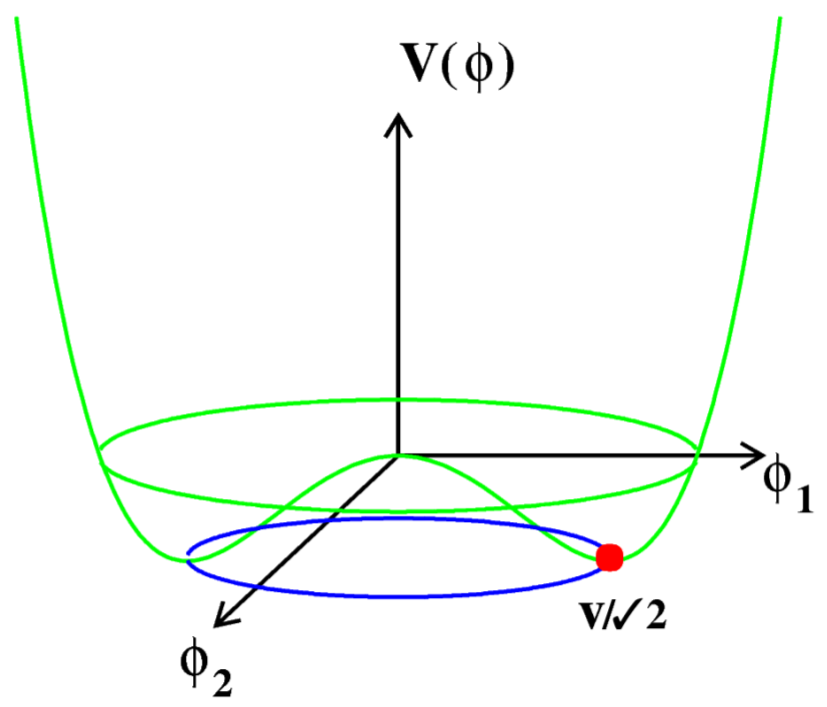
\includegraphics[width=0.5\textwidth]{./figures/theory/higgs_potential.png}
    \caption{Higgs potential for a scenario of spontaneous symmetry breaking. Only two degrees of freedom are shown~\cite{MarkusPhd}.}\label{fig:theory:sm:higgspotential}
\end{figure}

The Higgs potential can be minimized with respect to $\Phi^\dagger\Phi$ by
\begin{equation}
    \abs{\Phi_0}^2 = \frac{v}{\sqrt{2}} \,, v = \sqrt{\frac{\mu^2}{\lambda}} \,.
\end{equation}
Here, $v$ is the vacuum expectation value.
The usual choice of the ground state is $\Phi_1 = \Phi_2 = \Phi_4 = 0$ and $\Phi_3 = \abs{\Phi_0}$, which leads to
\begin{equation}
    \label{eq:theo:higgs:doublet}
    \Phi_0 = \frac{1}{\sqrt{2}}
    \begin{pmatrix}
        0 \\ v
    \end{pmatrix} \,.
\end{equation}
The ground state has the quantum numbers $Y = 0$ and $I_3 = - \frac{1}{2}$.
This breaks the $SU{(2)}_{L,I_w} \times U{(1)}_Y$ symmetry spontaneously to $U{(1)}_Q$.
However, the $U{(1)}_Q$ needs to remain unbroken, therefore $\Phi_1$ and $\Phi_2$ are set to zero, to obtain a neutral ground state.

The vacuum expectation value $v$ can bet set in relation to the Fermi constant $G_F$~\cite{PDG},
\begin{equation}
    v = {\left(\sqrt{2} G_F \right)}^{-\frac{1}{2}} = \SI{246}{\GeV} \,.
\end{equation}

To describe the potential around the ground state $\Phi_0$, the following parametrization can be made:
\begin{equation}
    \Phi(x) = \frac{1}{\sqrt{2}} \exp \left[ i \sum_{a=1}^{3} \frac{\tau_a G_a(x)}{v} \right]
    \begin{pmatrix}
         0 \\ v + H(x)
    \end{pmatrix} \,.
\end{equation}
Four new real scalar fields need to be introduced.
The three fields $G_a(x), (a=1,2,3)$ can be associated with the massless scalar Goldstone bosons~\cite{GoldstoneBoson1,GoldstoneBoson2}.
They can be eliminated by using a unitary gauge transformation of the form
\begin{equation}
    \Phi(x) \mapsto \Phi'(x) = \exp \left[ - i \sum_{a=1}^{3} \frac{\tau_a G_a(x)}{v} \right] \Phi(x) \,.
\end{equation}
The fourth field, $H(x)$, can be interpreted as an excitation of the ground state.
This excitation can be associated with a new scalar particle, the Higgs boson.

Using the definitions of the gauge boson fields from \cref{eq:theory:ew:zafield,eq:theory:ew:wfield}, the
Lagrangian density can be expanded as,
\begin{equation}
    \begin{split}
        \lagl_\text{Higgs} =& \frac{1}{2} (\partial_\mu H)(\partial^\mu H) - \lambda v^2 H^2 - \lambda v H^3 - \frac{1}{4} \lambda H^4 \\
        & + {\left(\frac{1}{2} v g \right)}^2 W^\mu_+ W^-_\mu + \frac{1}{2} {\left(\frac{v g}{2 \cos (\theta_w)}\right)}^2 Z^\mu Z_\mu \\
        & + g \left(\frac{v g }{2}\right) H W^\mu_+ W^-_\mu + g \frac{v g}{4 \cos^2 (\theta_w)} H Z^\mu Z_\mu \\
        & + \frac{g^2}{4} H^2 W^\mu_+ W^-_\mu + \frac{g^2}{4 \cos^2 (\theta_w)} H^2 Z^\mu Z_\mu + \text{const}.  \,.
    \end{split}
\end{equation}
The second line directly enables to read of the masses of the $W^\pm$- and $Z^0$-bosons\footnote{A mass term has generally a form of $\frac{1}{2}m^2 X^\mu X_\mu$ for a neutral particle
and $m^2 X^+ X^-$ for a charged particle, where $X$ denotes the field associated with the particle.},
\begin{equation}
    m_{W^\pm} = \frac{1}{2} v g \qquad \text{and} \qquad m_{Z^0} = \frac{v g }{2 \cos(\theta_w)} = \frac{m_{W^\pm}}{\cos(\theta_w)} \,.
\end{equation}
Therefore, the ratio of the masses of the $W^\pm$- and $Z^0$-bosons depends only on the weak mixing angle.

Furthermore, the mass of the Higgs is given by
\begin{equation}
    m_H = \sqrt{2\lambda} v \,.
\end{equation}

Additionally, the Lagrangian density contains cubic ($HVV$) and quartic ($HHVV$) terms, which describe
interactions between the Higgs boson and massive gauge bosons ($V$).
The coupling strength of the cubic and quartic interactions is proportional
to the mass of the gauge bosons, $m_{w^\pm}$ or $m_{Z^0}$, and the mass of the Higgs boson, $m_H$, respectively.
There are also cubic ($H^3$) and quartic ($H^4$) Higgs-boson self-interaction terms in the Lagrangian density.
All these couplings predicted by the spontaneous symmetry breaking enable to measure the relation between gauge boson
masses and coupling strengths.

Up to now only the gauge bosons and the Higgs boson acquire a mass.
Fermion masses can be included in the theory by introducing a new coupling, which has to be invariant under the $SU{(2)}_{L,I_w} \times U{(1)}_Y$.
The new coupling is called \emph{Yukawa coupling} and describes the coupling between left-handed fermion $SU{(2)}_{L,I_w}$-doublets,
right-handed fermion $U{(1)}_Y$-singles, and the Higgs-doublet.

For first-generation leptons the Lagrangian density of the Yukawa coupling is given by
\begin{equation}
    \lagl_\text{Yukawa}^\text{lep,1} = - g_e {(\overline{\nu}_e, \overline{e})}_L \Phi e_R + h.c. \,,
\end{equation}
where $h.c.$ denotes the corresponding hermitian conjugated term and $g_e$ the coupling strength.
Because of the form of the Higgs doublet $\Phi$ as defined in \cref{eq:theo:higgs:doublet} only the electron
acquires a mass, the neutrino remains massless.

Before the Yukawa coupling for quarks can defined, first an additional charge conjugated Higgs doublet $\Phi_C$
needs to be introduced, to enable couplings to quarks with $I_3 = \frac{1}{2}$,
\begin{equation}
    \Phi_C(x) = \frac{1}{\sqrt{2}}
    \begin{pmatrix}
        v + H(x) \\ 0
    \end{pmatrix} \,.
\end{equation}
Now, the Lagrangian density for the Yukawa coupling for quarks of the first generation can be written down,
\begin{equation}
    \lagl_\text{Yukawa}^\text{quark,1} = -g_d {(\overline{u}, \overline{d})}_L \Phi d_R - g_u {(\overline{u}, \overline{d})}_L \Phi_C u_R + h.c.
\end{equation}
For fermions of the second and third generation the same approach can be used.

It turns out that the coupling strength $g_f$ for fermions is directly proportional to the correspinding mass $m_f$ of the fermion,
\begin{equation}
    m_f  = v \frac{g_f}{\sqrt{2}} \,.
\end{equation}
If the excitation of the ground state is considered, the Lagrangian density of the Yukawa coupling to fermions can be written as
\begin{equation}
    \lagl_\text{Yukawa} = - m_f \overline{f} f \left(1 + \frac{H}{v}\right) \,.
\end{equation}

This is the last missing piece of the full Lagrangian density of the Standard Model,
\begin{equation}
    \lagl_\text{SM} = \lagl_\text{QCD} + \lagl_\text{EW} + \lagl_\text{Higgs} + \lagl_\text{Yukawa} \,.
\end{equation}
The only unknown parameter is $\lambda$, since all other paraters are fixed by the masses of the gauge bosons and fermions, which
can be experimentally measured.
Thus, $\lambda$ needs to be determined by measuring the mass of the Higgs boson.

\section{The Higgs Boson}\label{sec:theory:higgs}

The Higgs boson was predicted by the Higgs mechanism in Standard Model since the 1960s.
It has no electric or color charge and has a spin-parity configuration of $J^{CP} = 0^+$.
Its mass is not predicted and con only be determined by experiments.
The coupling strength is proportional to the mass of fermions and proportional to the squared mass of gauge bosons.

In 2012 the Higgs boson was observed with the ATLAS and CMS experiments at CERN~\cite{HiggsDiscoveryATLAS,HiggsDiscoveryCMS} with a
mass of $m_H = \SI{125}{\GeV}$.
Due to its short lifetime of about $\SI{e-22}{\s}$ it cannot be observed directly, but only via its decay products.
Because the cross-section of the Higgs boson is several magnitudes smaller than the ones from other processes produced at the LHC,
as can be seen in \cref{fig:theory:higgs:smxsec}, refined analysis strategies are needed.
In this section the production of the Higgs boson at the LHC is discussed, followed by an overview of the decay modes of the Higgs boson.
Measurements of the properties of the Higgs boson are discussed in \cref{sec:theory:measurements}.

\begin{figure}[htb]
    \centering
    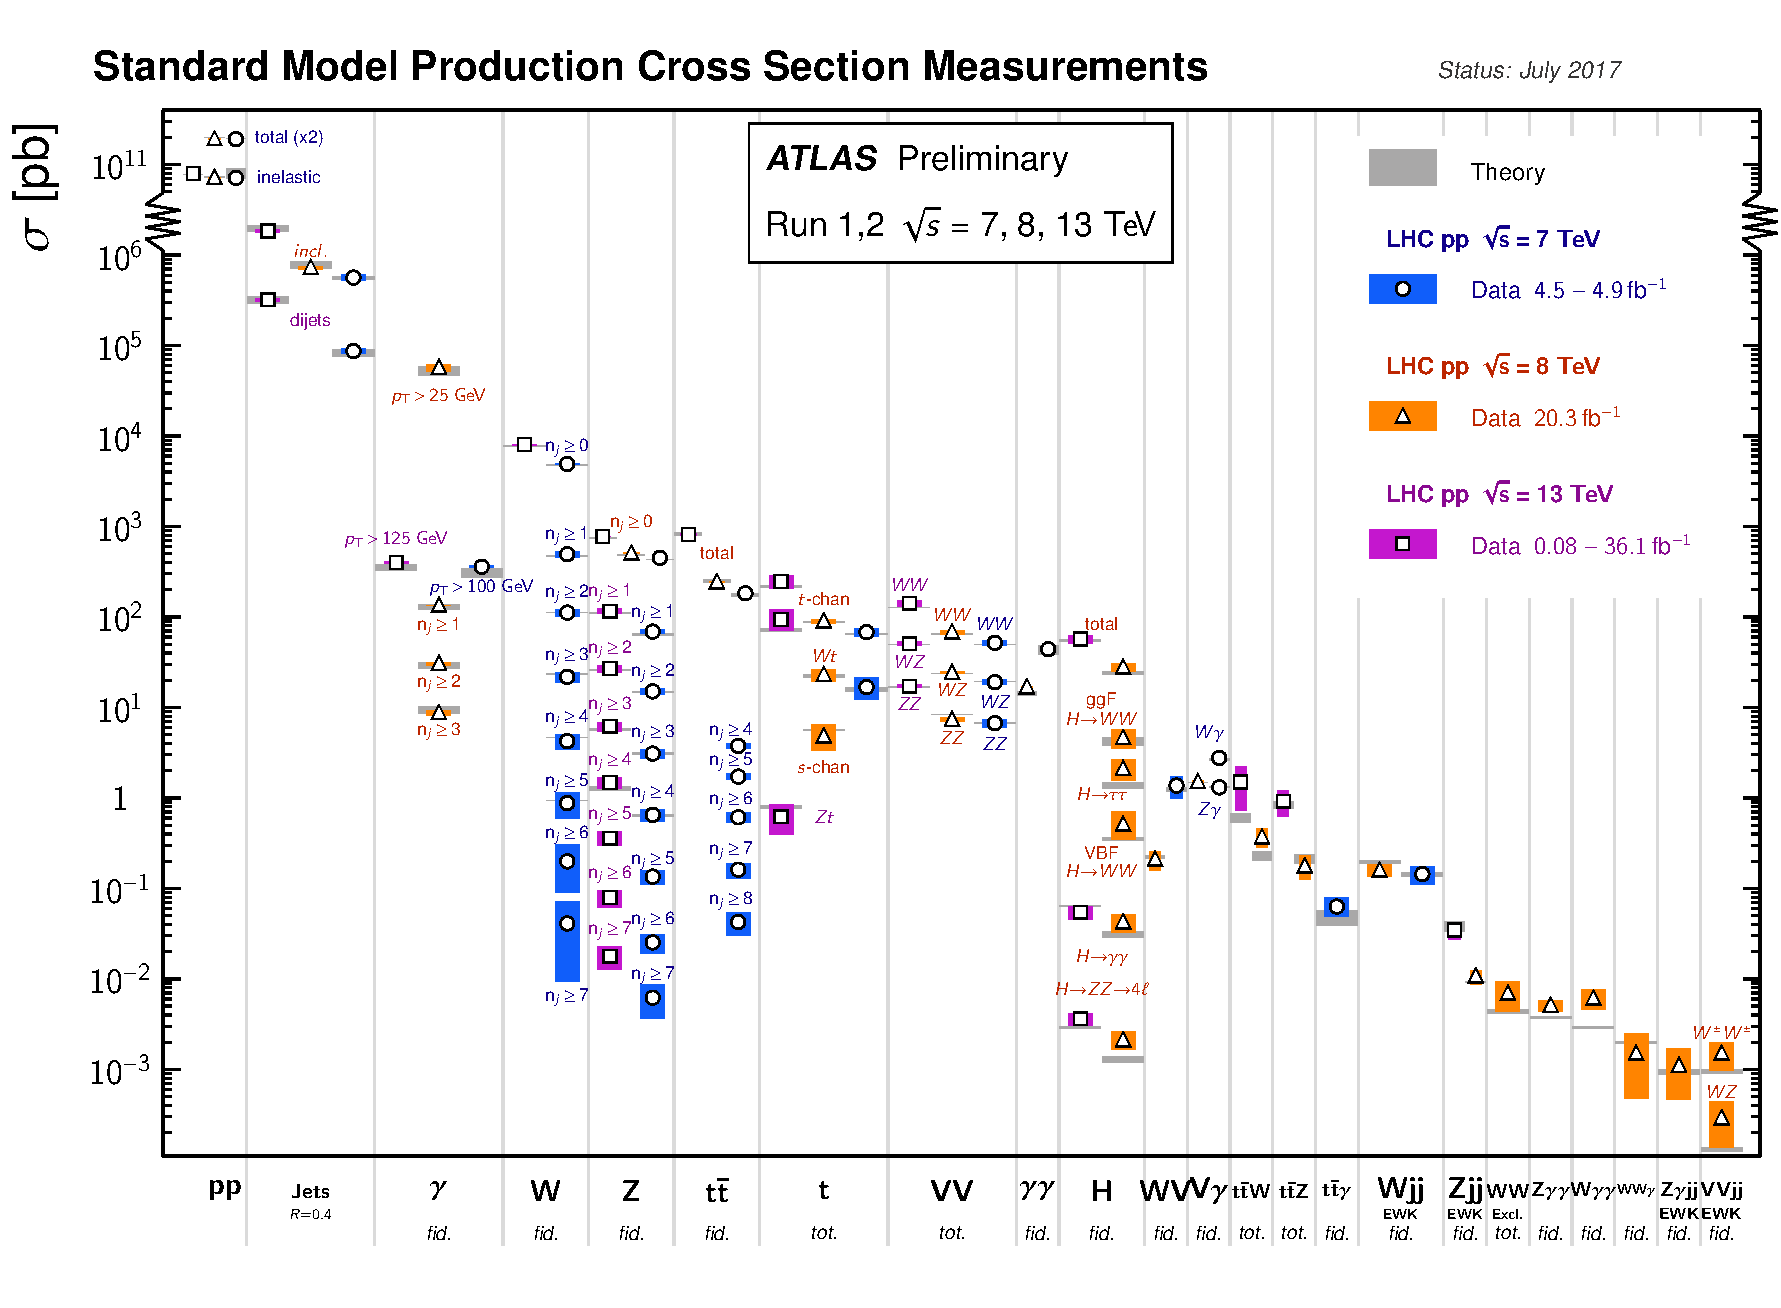
\includegraphics[width=0.9\textwidth]{./figures/theory/sm_xsec.eps}
    \caption{Overview of inclusive and fiducial SM cross-sections measured during Run-1 and Run-2 and compared to theory predictions~\cite{SMPublicResults}.}\label{fig:theory:higgs:smxsec}
\end{figure}

\subsection{Higgs Boson Production in Proton--Proton Collisions}\label{sub:theory:higgs:production}

In proton--proton collisions at the LHC the constituents of the protons can be described as free, charged, point-like particles, which are called \emph{partons}.
The possibility to find a parton with a momentum fraction $x$ of the total momentum of the proton is given
by the parton distribution function (PDF), $f(x_i, Q^2)$, which depends on the squared momentum transfer, $Q^2$.
To calculate the cross-section of the production of a particle $X$ in proton--proton collisions the
cross-section at parton level $\hat{\sigma}_{ij\to X}$ has to be weighted with the PDFs and all
possible momentum fractions need to be considered, as prescribed by the factorization theorem~\cite{DRELL1971578}.
Mathematically speaking this is a convolution of the PDFs with the partonic cross-section,
\begin{equation}
    \sigma_{X} = \sum_{i,j} \int_{0}^{1} \dif x_i \int_{0}^{1} \dif x_j \,
    f_i \left( x_i , \mu_F^2 \right) f_j \left( x_j , \mu_f^2 \right) \hat{\sigma}_{ij\to X} (\alpha_s, \mu_R^2) \,,
\end{equation}
where $\mu_F$ is the factorization scale and $\mu_F$ the renormalization scale.
The general expression for the partonic cross-section is~\cite{Griffiths}
\begin{equation}
    \hat{\sigma}_{ij\to X} = \frac{1}{F} \int \matrixm \left(ij \to X \right) \dif \Phi \,,
\end{equation}
with the matrix element $\matrixm$ which describes the transition probability of the initial state $ij$ to the final state $X$, the
particle flux $F$, and the phase-space factor $\dif \Phi$ depending on the kinematics of the collision.
\\[\baselineskip]
The Higgs boson can be produced in multiple ways, which vary in cross-section and phenomenology.
In \cref{fig:theory:higgs:production} the leading order (LO) Feynman diagrams are shown for the dominant production modes
at the LHC\@.

\begin{figure}[htb]
    \centering
    \begin{subfigure}[t]{0.302\textwidth}
        \includegraphics[width=\textwidth]{feynman/h_ggf.pdf}
        \caption{gluon--gluon fusion}\label{fig:theory:higgs:ggf}
    \end{subfigure}
    \begin{subfigure}[t]{0.201\textwidth}
        \captionsetup{justification=raggedright}
        \includegraphics[width=\textwidth]{feynman/h_vbf.pdf}
        \caption{vector boson fusion}\label{fig:theory:higgs:vbf}
    \end{subfigure}
    \begin{subfigure}[t]{0.201\textwidth}
        \includegraphics[width=\textwidth]{feynman/h_strahl.pdf}
        \caption{Higgs-Strahlung}\label{fig:theory:higgs:vh}
    \end{subfigure}
    \begin{subfigure}[t]{0.246\textwidth}
        \captionsetup{justification=raggedright}
        \includegraphics[width=\textwidth]{feynman/h_top.pdf}
        \caption{associated \mbox{production} with top-quarks}\label{fig:theory:higgs:tassoc}
    \end{subfigure}
    \caption{Feynman diagrams of the dominant production modes of the Higgs boson at the LHC\@. The cross-section
             decreases from left to right.}\label{fig:theory:higgs:production}
\end{figure}

The production mode with the highest cross-section is gluon--gluon fusion (ggF).
This is caused by the high contribution of the gluon PDF in protons for small momentum fractions $x$, which enables
a quark loop producing a Higgs boson. Because coupling strength of the Higgs boson is proportional to the mass of the
interaction particle, top and bottom quarks contributions dominate in the quark loop.
At leading order only the Higgs boson is produced, therefore it has no transverse momentum.
However, at higher orders final state QCD radiation is possible, which acts as a recoil partner for the Higgs boson.
This is important for measurements to reduce background contributions.

The cross-section of the vector-boson fusion (VBF) production mode is one order below the one of gluon--gluon fusion.
Here two initial state quarks radiate a $Z^0$ or $W^\pm$ boson.
The bosons annihilate and produce a Higgs boson.
The two final state quarks provide a characteristic signature, which is defined by a high mass of the dijet system
and a large separation of the two jets in the pseudorapidity $\eta$ as defined in \cref{eq:pseudorapidity}.

Another production mode is the so-called Higgs-Strahlung, where one weak boson created by the annihilation of
a quark--antiquark pair radiates a Higgs boson.

The Higgs boson production associated with a top-quark pair has a suppressed cross-section compared with the
other production modes.
Because of the large mass of the top quark a high invariant mass is required, which reduces the available phase space.

A distribution of the cross-sections for different Higgs-boson production-modes as a function of the center-of-mass
energy $\sqrt{s}$ is shown in \cref{fig:theory:higgs:xsecs}.
The values of the cross-sections of the most dominant production modes of the Higgs boson at $\sqrt{s} = \SI{13}{\GeV}$
and corresponding uncertainties are listed in \cref{tab:theory:higgs:prodxsec}.

\begin{figure}[htb]
    \centering
    \begin{subfigure}[t]{0.45\textwidth}
        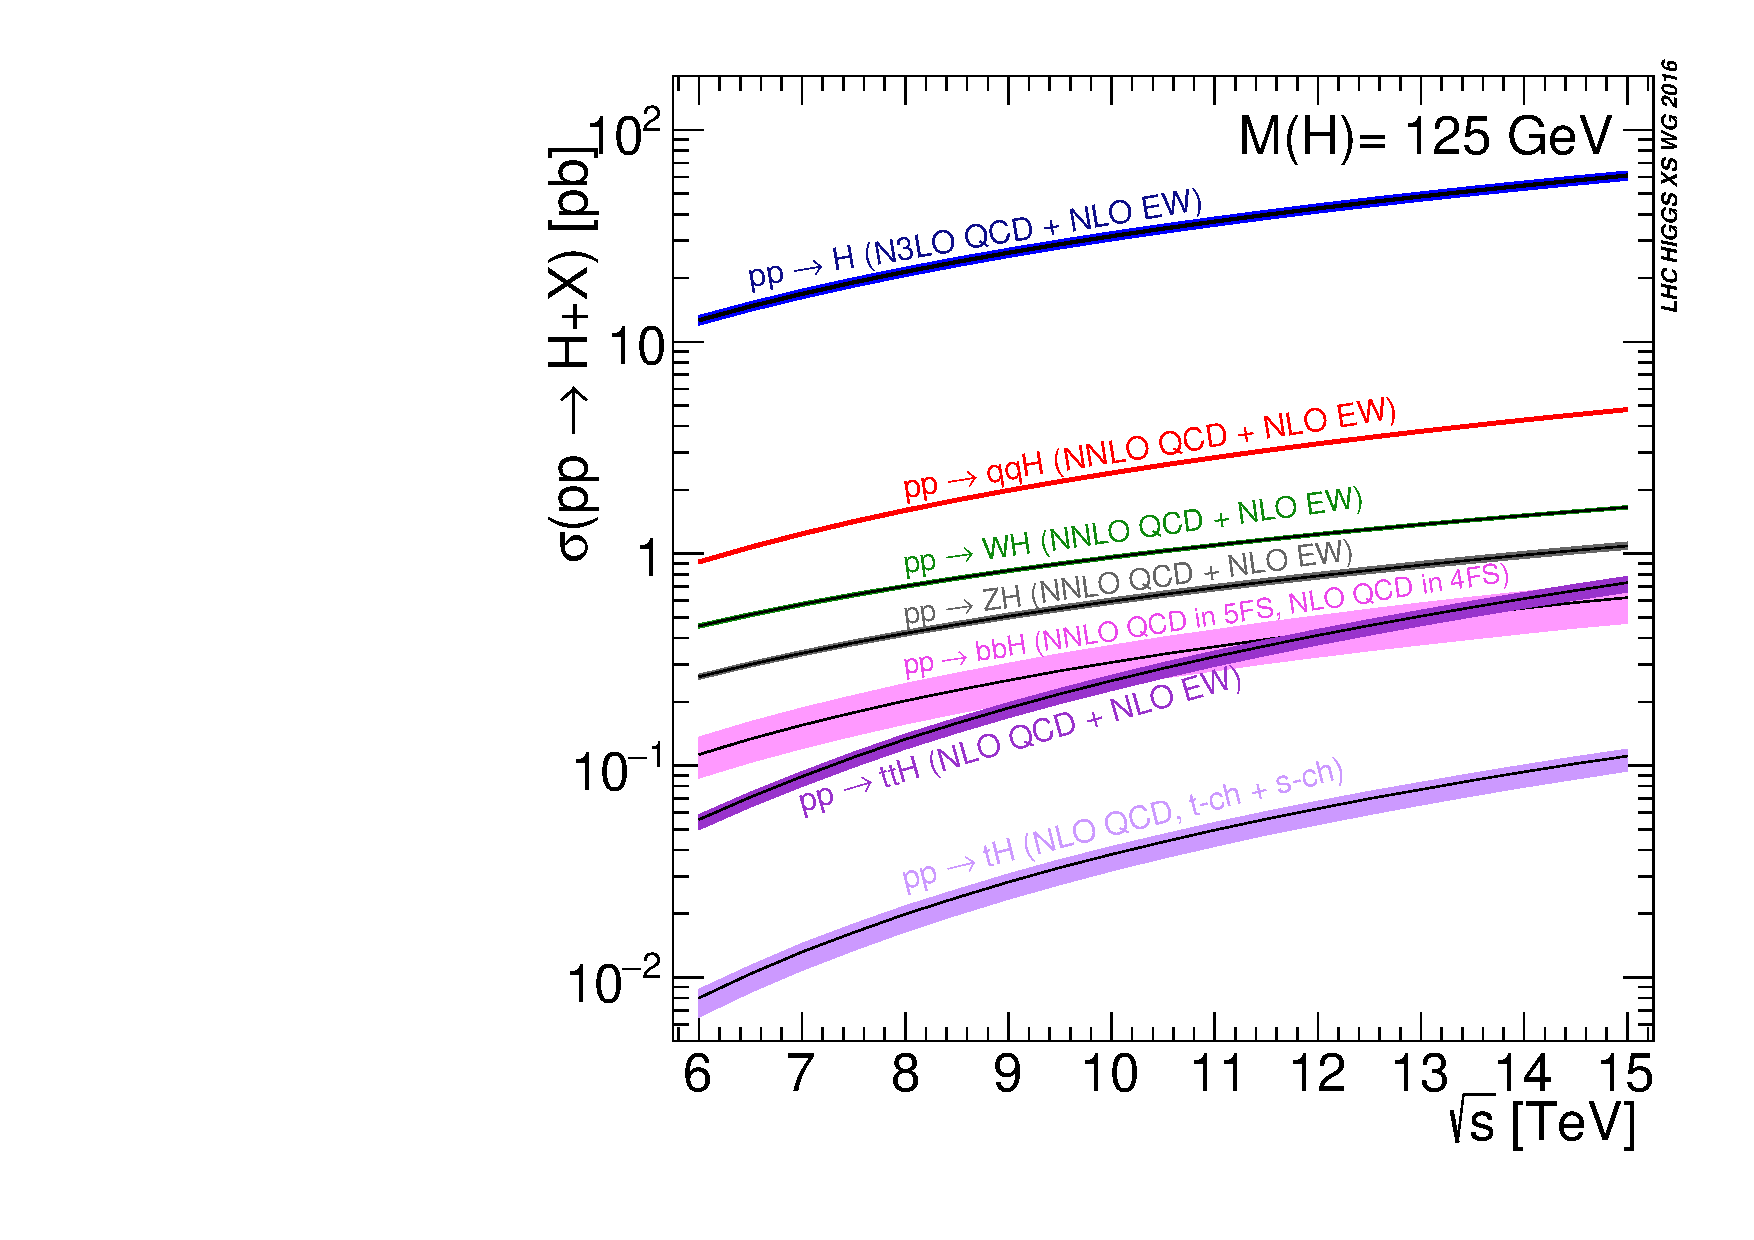
\includegraphics[width=\textwidth]{./figures/theory/higgs_xsec_production.pdf}
        \caption{Production cross-sections.}\label{fig:theory:higgs:xsecs}
    \end{subfigure}
    \begin{subfigure}[t]{0.45\textwidth}
        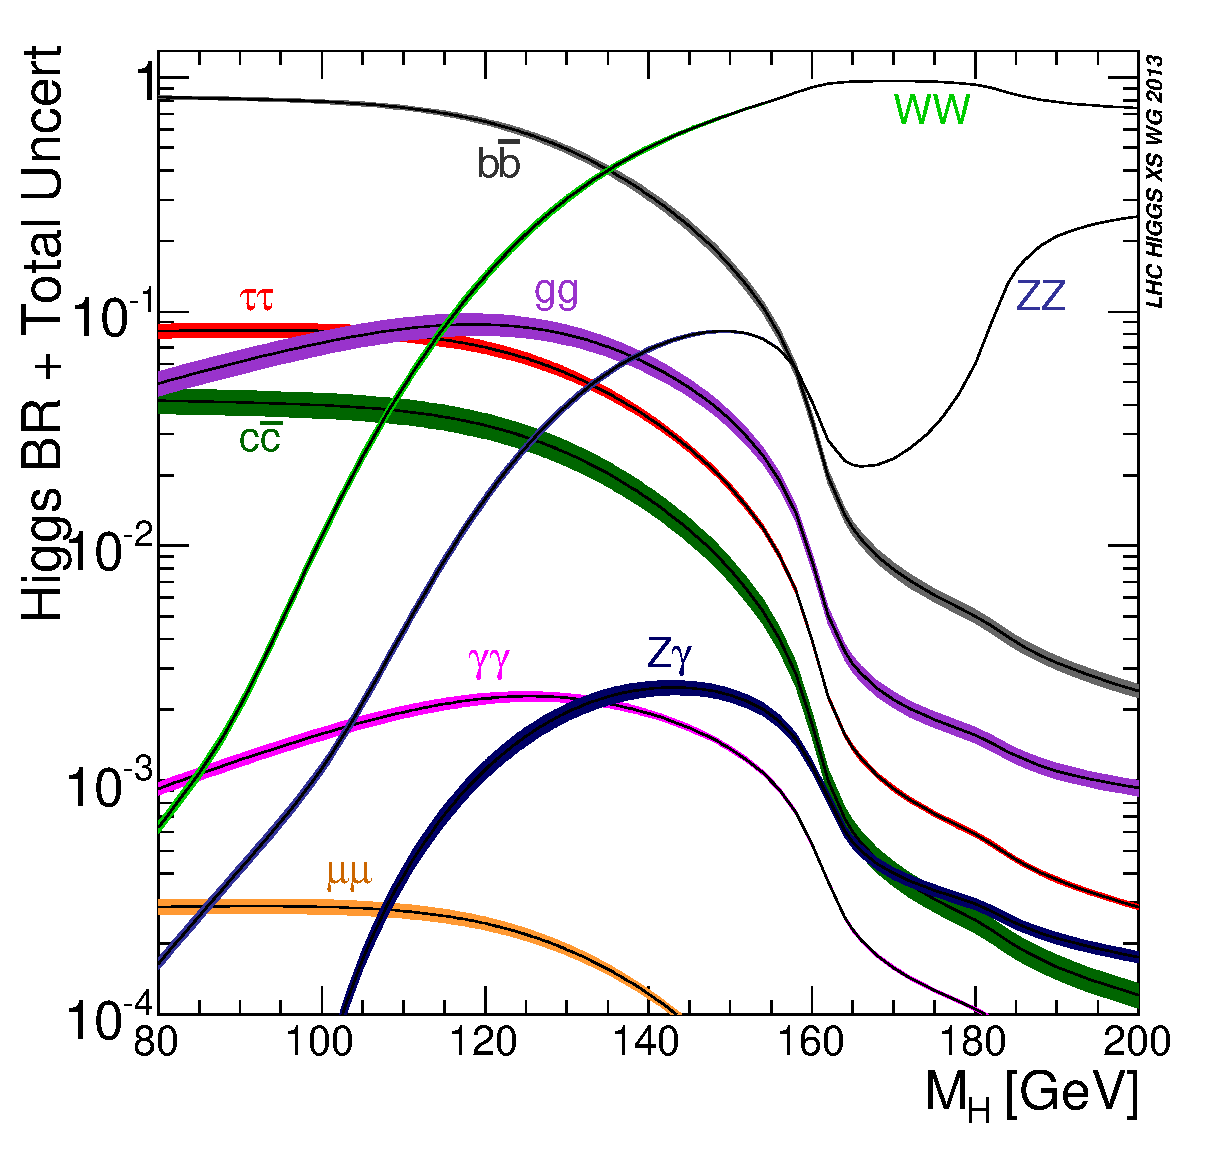
\includegraphics[width=\textwidth]{./figures/theory/higgs_xsec_decay.eps}
        \caption{Decay modes.}\label{fig:theory:higgs:br}
    \end{subfigure}
    \caption{Production cross-sections of the Higgs boson as a function of the center-of-mass energy $\sqrt{s}$ (a)~\cite{YR4}
             and branching ratios of the Higgs boson decay-modes depending in the mass $m_H$ of the Higgs boson (b)~\cite{YR3}.}
\end{figure}

\begin{table}[htpb]
    \centering
    \caption{Cross-sections for different production modes of the Higgs boson with different uncertainties
             for proton--proton collisions at $\sqrt{s} = \SI{13}{\TeV}$ and a mass of the Higgs boson
             of $m_H = \SI{125}{\GeV}$. Additionally the fraction with respect to the total cross section of the Higgs boson, $\sigma_i / \sigma_\text{tot}$, is given~\cite{YR4}.}\label{tab:theory:higgs:prodxsec}
    \begin{tabular}{cScSSS}
        \toprule
        Mode & $\sigma / \si{\pico\barn}$ & $\delta_\text{QCD scale}$ & $\delta_\text{PDF}$ & $\delta_{\alpha_s}$ & {$\sigma_i / \sigma_\text{tot}$} \\ \midrule
        ggF & 48.58 & \errud{\SI{4.6}{\percent}}{\SI{6.7}{\percent}} & \SI{\pm 1.9}{\percent} & \SI{\pm 2.6}{\percent}  & \SI{88}{\percent} \\ \addlinespace[0.2em]
        VBF & 3.782 & \errud{\SI{0.4}{\percent}}{\SI{0.3}{\percent}} & \SI{\pm 2.1}{\percent} & \SI{\pm 0.5}{\percent}  & \SI{6.7}{\percent} \\ \addlinespace[0.2em]
        WH  & 1.373 & \errud{\SI{0.5}{\percent}}{\SI{0.7}{\percent}} & \SI{\pm 1.7}{\percent} & \SI{\pm 0.9}{\percent}  & \SI{2.5}{\percent} \\ \addlinespace[0.2em]
        ZH  & 0.8839 & \errud{\SI{3.8}{\percent}}{\SI{3.1}{\percent}} & \SI{\pm 1.3}{\percent} & \SI{\pm 0.9}{\percent} & \SI{1.60}{\percent}  \\ \addlinespace[0.2em]
        ttH & 0.5071 & \errud{\SI{5.8}{\percent}}{\SI{9.2}{\percent}} & \SI{\pm 3.0}{\percent} & \SI{\pm 2.0}{\percent} & \SI{0.92}{\percent}  \\
        \bottomrule
    \end{tabular}
\end{table}

\subsection{Decay Modes of the Higgs Boson}
\label{sub:theory:higgs:decay}

The coupling strengths $m_f/v$ and $m_V^2/v$ of the Higgs-boson coupling to fermions $f$ and gauge bosons $V$ are proportional to the masses
of the interacting particles.
Thus, the branching ratio (BR), which is defined as the fraction of partial decay width to the total decay width,
\begin{equation}
    BR(H\to X) = \frac{\Gamma(H\to X)}{\Gamma_\text{total}} \,,
\end{equation}
increasing for higher masses of the decaying particles.

The dominant decay channels for fermions are $H\to b \overline{b}$, $H \to \tau^+\tau^-$, $H \to c\overline{c}$, and $H \to \mu^+\mu^-$.
Furthermore, the Higgs boson can decay directly into massive gauge bosons, $H \to WW^*$ and $H \to ZZ^*$.
Using a heavy quark loop and $W$-boson loop, it can also decay into massless gauge bosons, $H \to gg$ and $H \to \gamma\gamma$.

The branching ratios depending on the mass of the Higgs boson are shown in \cref{fig:theory:higgs:br}.
The corresponding values for a Higgs boson with a mass $m_H = \SI{125}{\GeV}$ are listed in \cref{tab:theory:higgs:br}.
At the LHC the two most dominant decay modes are the decay into
a bottom-quark pair with a branching ratio of \SI{58.24}{\percent} and the decay into a pair of $W$-bosons with a BR
of \SI{21.37}{\percent}.
The focus of this analysis is on the decay into a pair of $\tau$-leptons, which has a branching ratio of \SI{6.272}{\percent}.

\begin{table}[htpb]
    \centering
    \caption{Branching ratios for various decay modes of the Higgs boson with a mass of $m_H = \SI{125}{\GeV}$
    with corresponding theoretical uncertainties (THU) and parametric uncertainties from the quark masses (PU($m_q$)) and the strong coupling constant (PU($\alpha_S$))
    expressed in percent~\cite{YR4}.}\label{tab:theory:higgs:br}
    \begin{tabular}{cSccc}
        \toprule
        Decay channel       & {Branching Ratio [\%]} & THU [\%] & PU($m_q$) [\%] & PU($\alpha_s$) [\%] \\ \midrule
        $b \overline{b}$    & 58.24   & \errud{0.65}{0.65} & \errud{0.72}{0.74} & \errud{0.78}{0.80} \\
        $WW$                & 21.37   & \errud{0.99}{0.99} & \errud{0.99}{0.98} & \errud{0.66}{0.63} \\
        $gg$                & 8.187   & \errud{3.40}{3.41} & \errud{1.12}{1.13} & \errud{3.69}{3.61} \\
        $\tau^+\tau^-$      & 6.272   & \errud{1.17}{1.16} & \errud{0.98}{0.99} & \errud{0.62}{0.62} \\
        $c\overline{c}$     & 2.891   & \errud{1.20}{1.20} & \errud{5.26}{0.98} & \errud{1.25}{1.25} \\
        $ZZ$                & 2.619   & \errud{0.99}{0,99} & \errud{0.99}{0.98} & \errud{0.66}{0.63} \\
        $\gamma\gamma$      & 0.2270  & \errud{1.73}{1.72} & \errud{0.93}{0.99} & \errud{0.61}{0.62} \\
        $Z\gamma$           & 0.1533  & \errud{5.71}{5.71} & \errud{0.98}{1.01} & \errud{0.58}{0.65} \\
        $\mu^+\mu^-$        & 0.02176 & \errud{1.23}{1.23} & \errud{0.97}{0.99} & \errud{0.59}{0.64} \\
        \bottomrule
    \end{tabular}
\end{table}
\section{Measurements of the Higgs Boson at the LHC}\label{sec:theory:measurements}

This section gives an overview of recent measurements of Higgs-boson properties during Run-1 and Run-2 of the LHC\@.

\subsection{Discovery}\label{sub:theory:meas:discovery}

The observation of a new particle with a mass of \SI{125}{\GeV} in the search for a SM Higgs-boson was
announced by both the ATLAS and CMS experiment on \nth{4} of July 2012~\cite{HiggsDiscoveryATLAS,HiggsDiscoveryCMS}.
The observed significance was $5.9\sigma$ and $5.0\sigma$ for ATLAS and CMS, respectively, which is passing the threshold of $5\sigma$
needed for an observation.
The $p_0$ values as a function of the mass of the Higgs boson can be seen in \cref{fig:theory:meas:disc:p0}.
Results from the $H\to\gamma\gamma$, $H\to ZZ$, $H \to WW$, $H\to\tau\tau$, $H\to b\overline{b}$ decay channels were used for the observation.\footnote{The $H\to b\overline{b}$ channel was only used by CMS.}

\begin{figure}[htb]
    \centering
    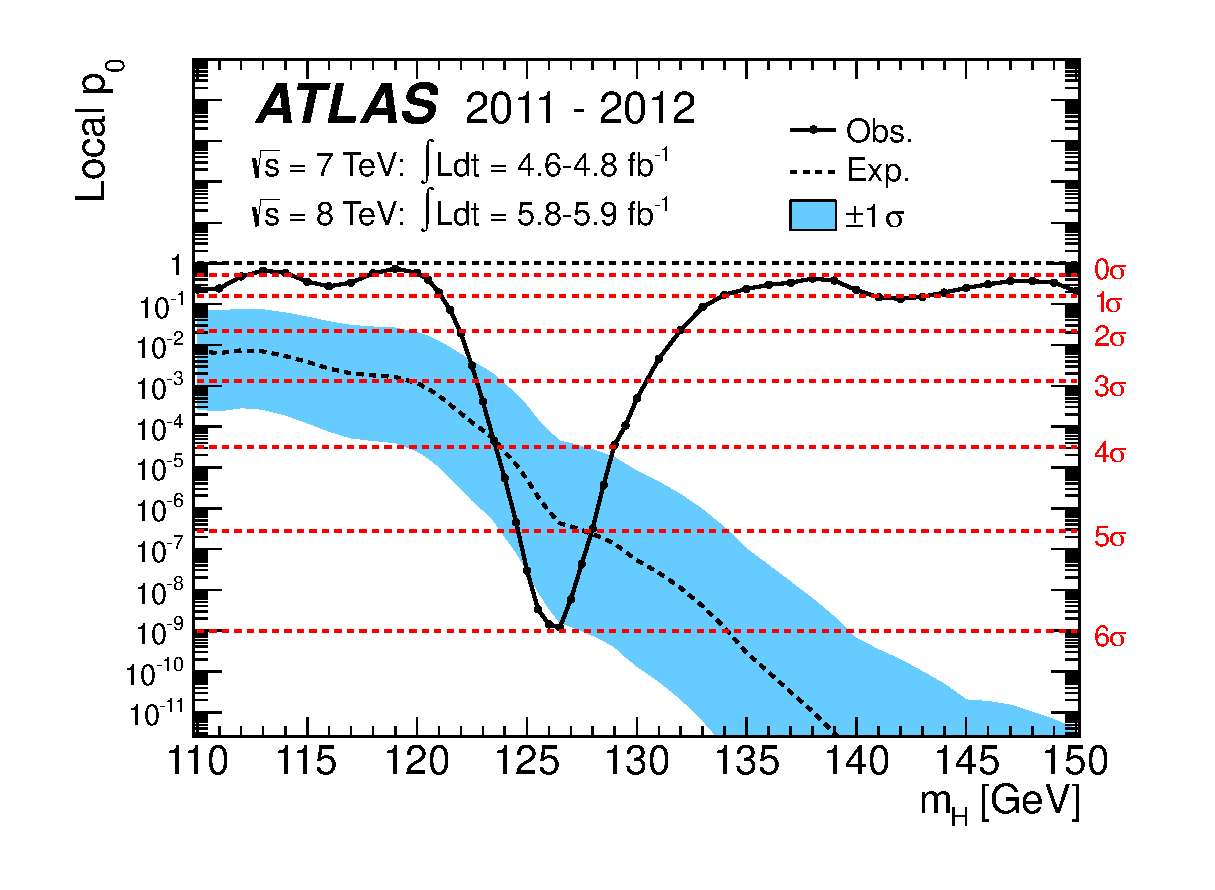
\includegraphics[width=0.45\textwidth]{./figures/theory/atlas_higgs_p0.eps}
    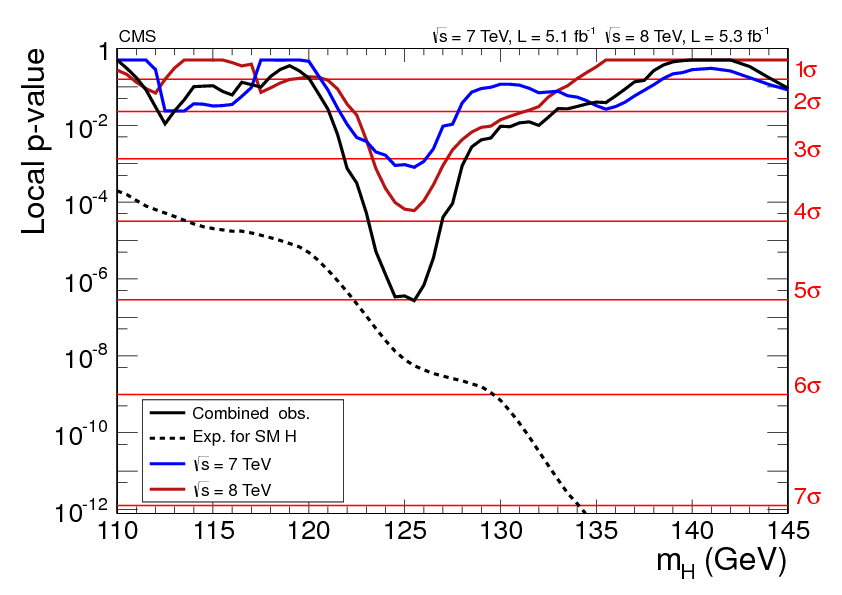
\includegraphics[width=0.45\textwidth]{./figures/theory/cms_higgs_p0.png}
    \caption{Values for $p_0$ depending on the mass of the Higgs boson, $m_H$, from the observation of the
             Higgs boson during Run-1 with the ATLAS (left,~\cite{HiggsDiscoveryATLAS}) and CMS (right,~\cite{HiggsDiscoveryCMS}) experiments.
             The black dashed lines show the expected values.
             The corresponding significances are indicated by red lines.}\label{fig:theory:meas:disc:p0}
\end{figure}

\subsection{Measurements during Run-1}\label{sub:theory:meas:run1}

During Run-1 several properties of Higgs boson were measured, like the mass, signal strength, decay width, as well as
spin and CP properties.

\subsubsection{Mass measurement}\label{subsub:theory:meas:run1:mass}

The mass of the Higgs boson was determined individually by the ATLAS and CMS experiment and
in a combined measurement using the full Run-1 dataset.
For the mass measurement only the $H\to\gamma\gamma$ and $H\to ZZ \to 4\ell$ channels were used, since other channels
provide a worse mass resolution or do not have direct access to the mass of the Higgs boson.
The combined result is~\cite{MassCombinedMeas}
\begin{equation}
    m_H = (125.09 \pm 0.21 \text{(stat.)} \pm 0.11 \text{(sys.)})\,\text{GeV} \,,
\end{equation}
individual results are shown in \cref{fig:theory:meas:run1:mass}.

\begin{figure}[htb]
    \centering
    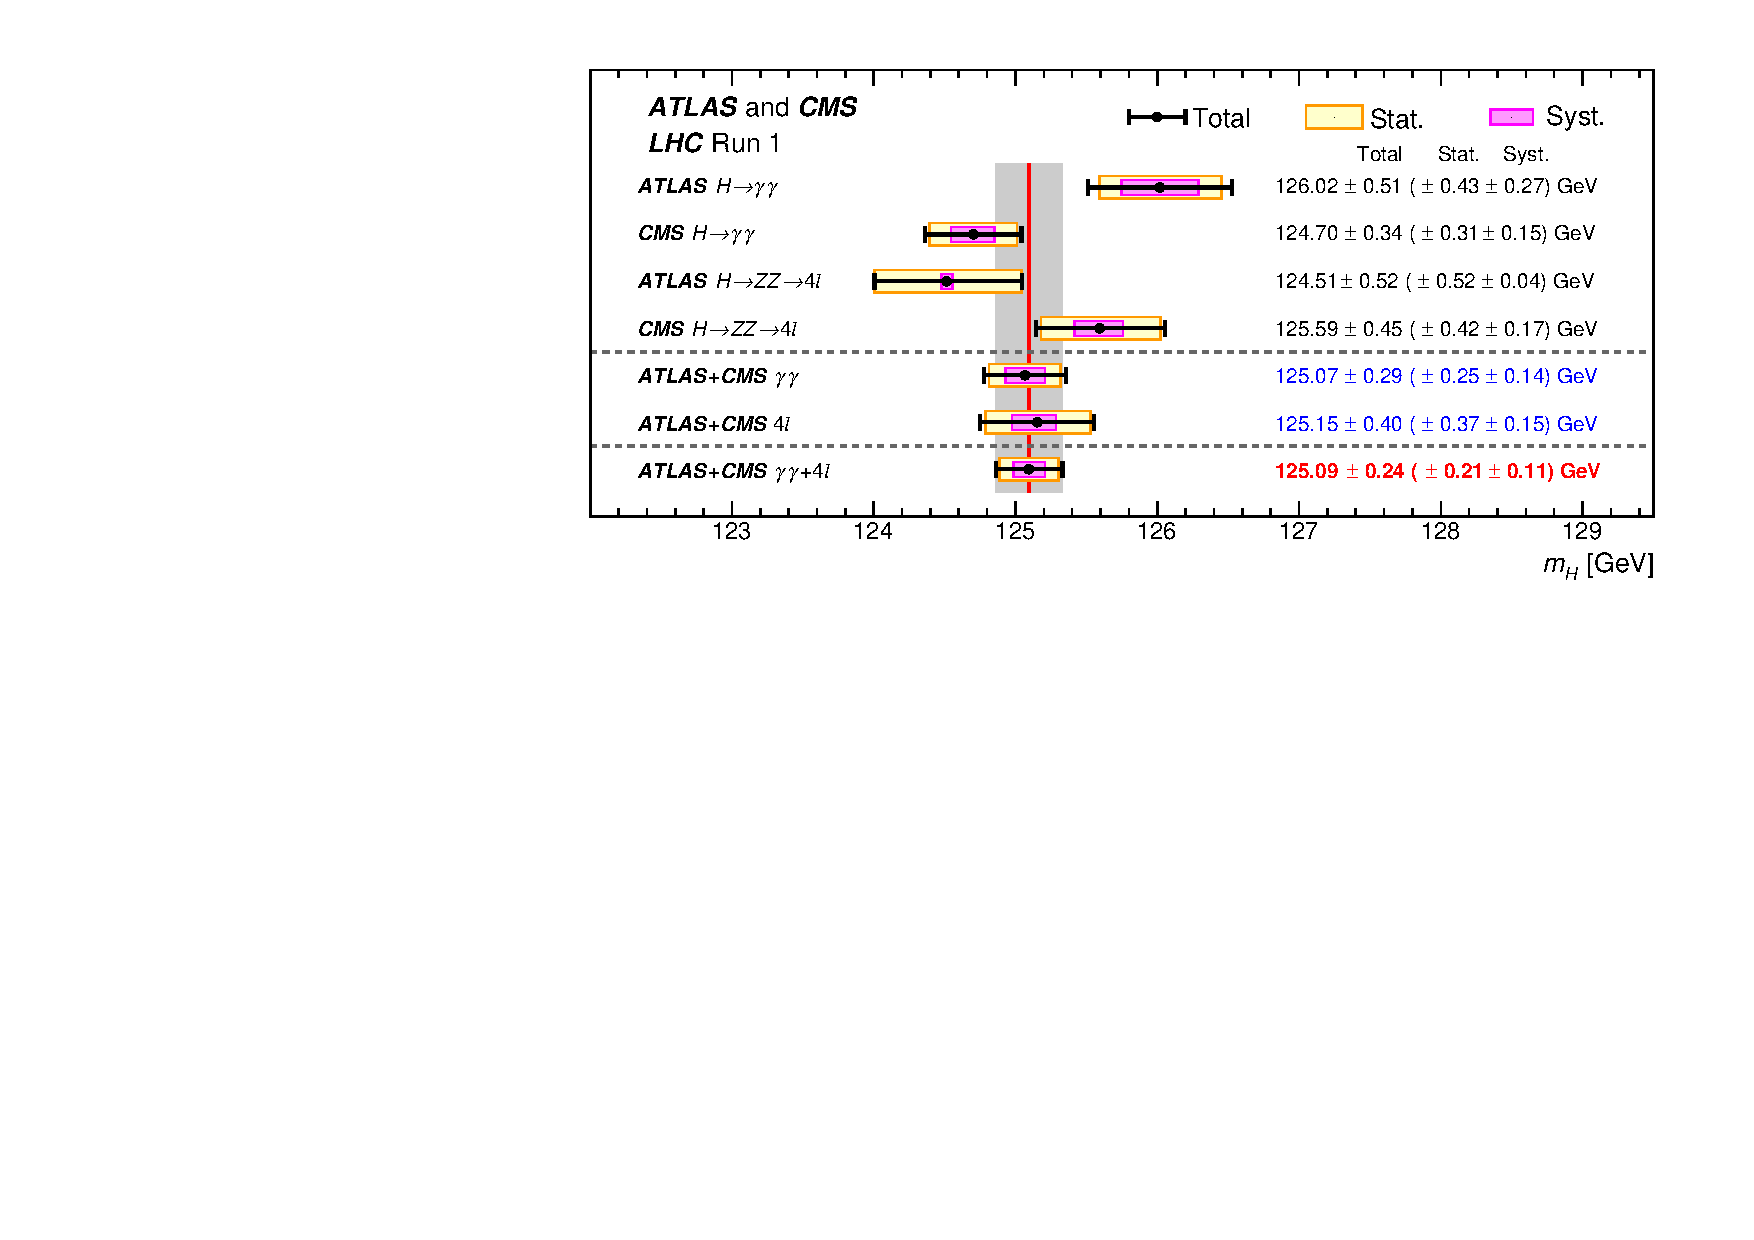
\includegraphics[width=0.9\textwidth]{./figures/theory/mass_combination_atlascms.pdf}
    \caption{Measurement of the mass of the Higgs boson in the $H\to\gamma\gamma$ and $H \to ZZ \to 4\ell$ decay channels during Run-1 with the ATLAS and CMS detector~\cite{MassCombinedMeas}.}\label{fig:theory:meas:run1:mass}
\end{figure}

\subsubsection{Signal strength}\label{subsub:theory:meas:run1:mu}

The measured cross section of a process is usually not given directly, but the ratio of the measured cross section
to the prediction of the SM is used,
\begin{equation}
    \label{eq:theo:mu}
    \mu = \frac{\sigma_\text{experimental}}{\sigma_\text{SM}} \,.
\end{equation}
This ratio is the so-called \emph{signal strength} and is denoted with $\mu$.
This makes it very easy to check if the measured cross section is in agreement with the standard model value for different processes, which would be
always indicated by $\mu = 1$.

The signal strength of the Higgs boson can be determined for different production modes and decay channels, as shown in \cref{fig:theory:meas:run1:mu}.
Since the signal strength is the product of the production and decay signal strength,
the decay cross sections are assumed to be $\pm1$ for the measurement of the production cross sections and vice versa.
All signal strengths agree within uncertainties with the predicted SM value of $\mu = 1$.
The combined signal strength is~\cite{HiggsMuCombined}
\begin{equation}
    \mu = 1.09 \pm  0.07 \text{(stat.)} \errud{0.09}{0.08} \text{(sys.)} \,,
\end{equation}
which matches with the SM expectation within the uncertainties.

\begin{figure}[htb]
    \centering
    \begin{subfigure}[c]{0.45\textwidth}
        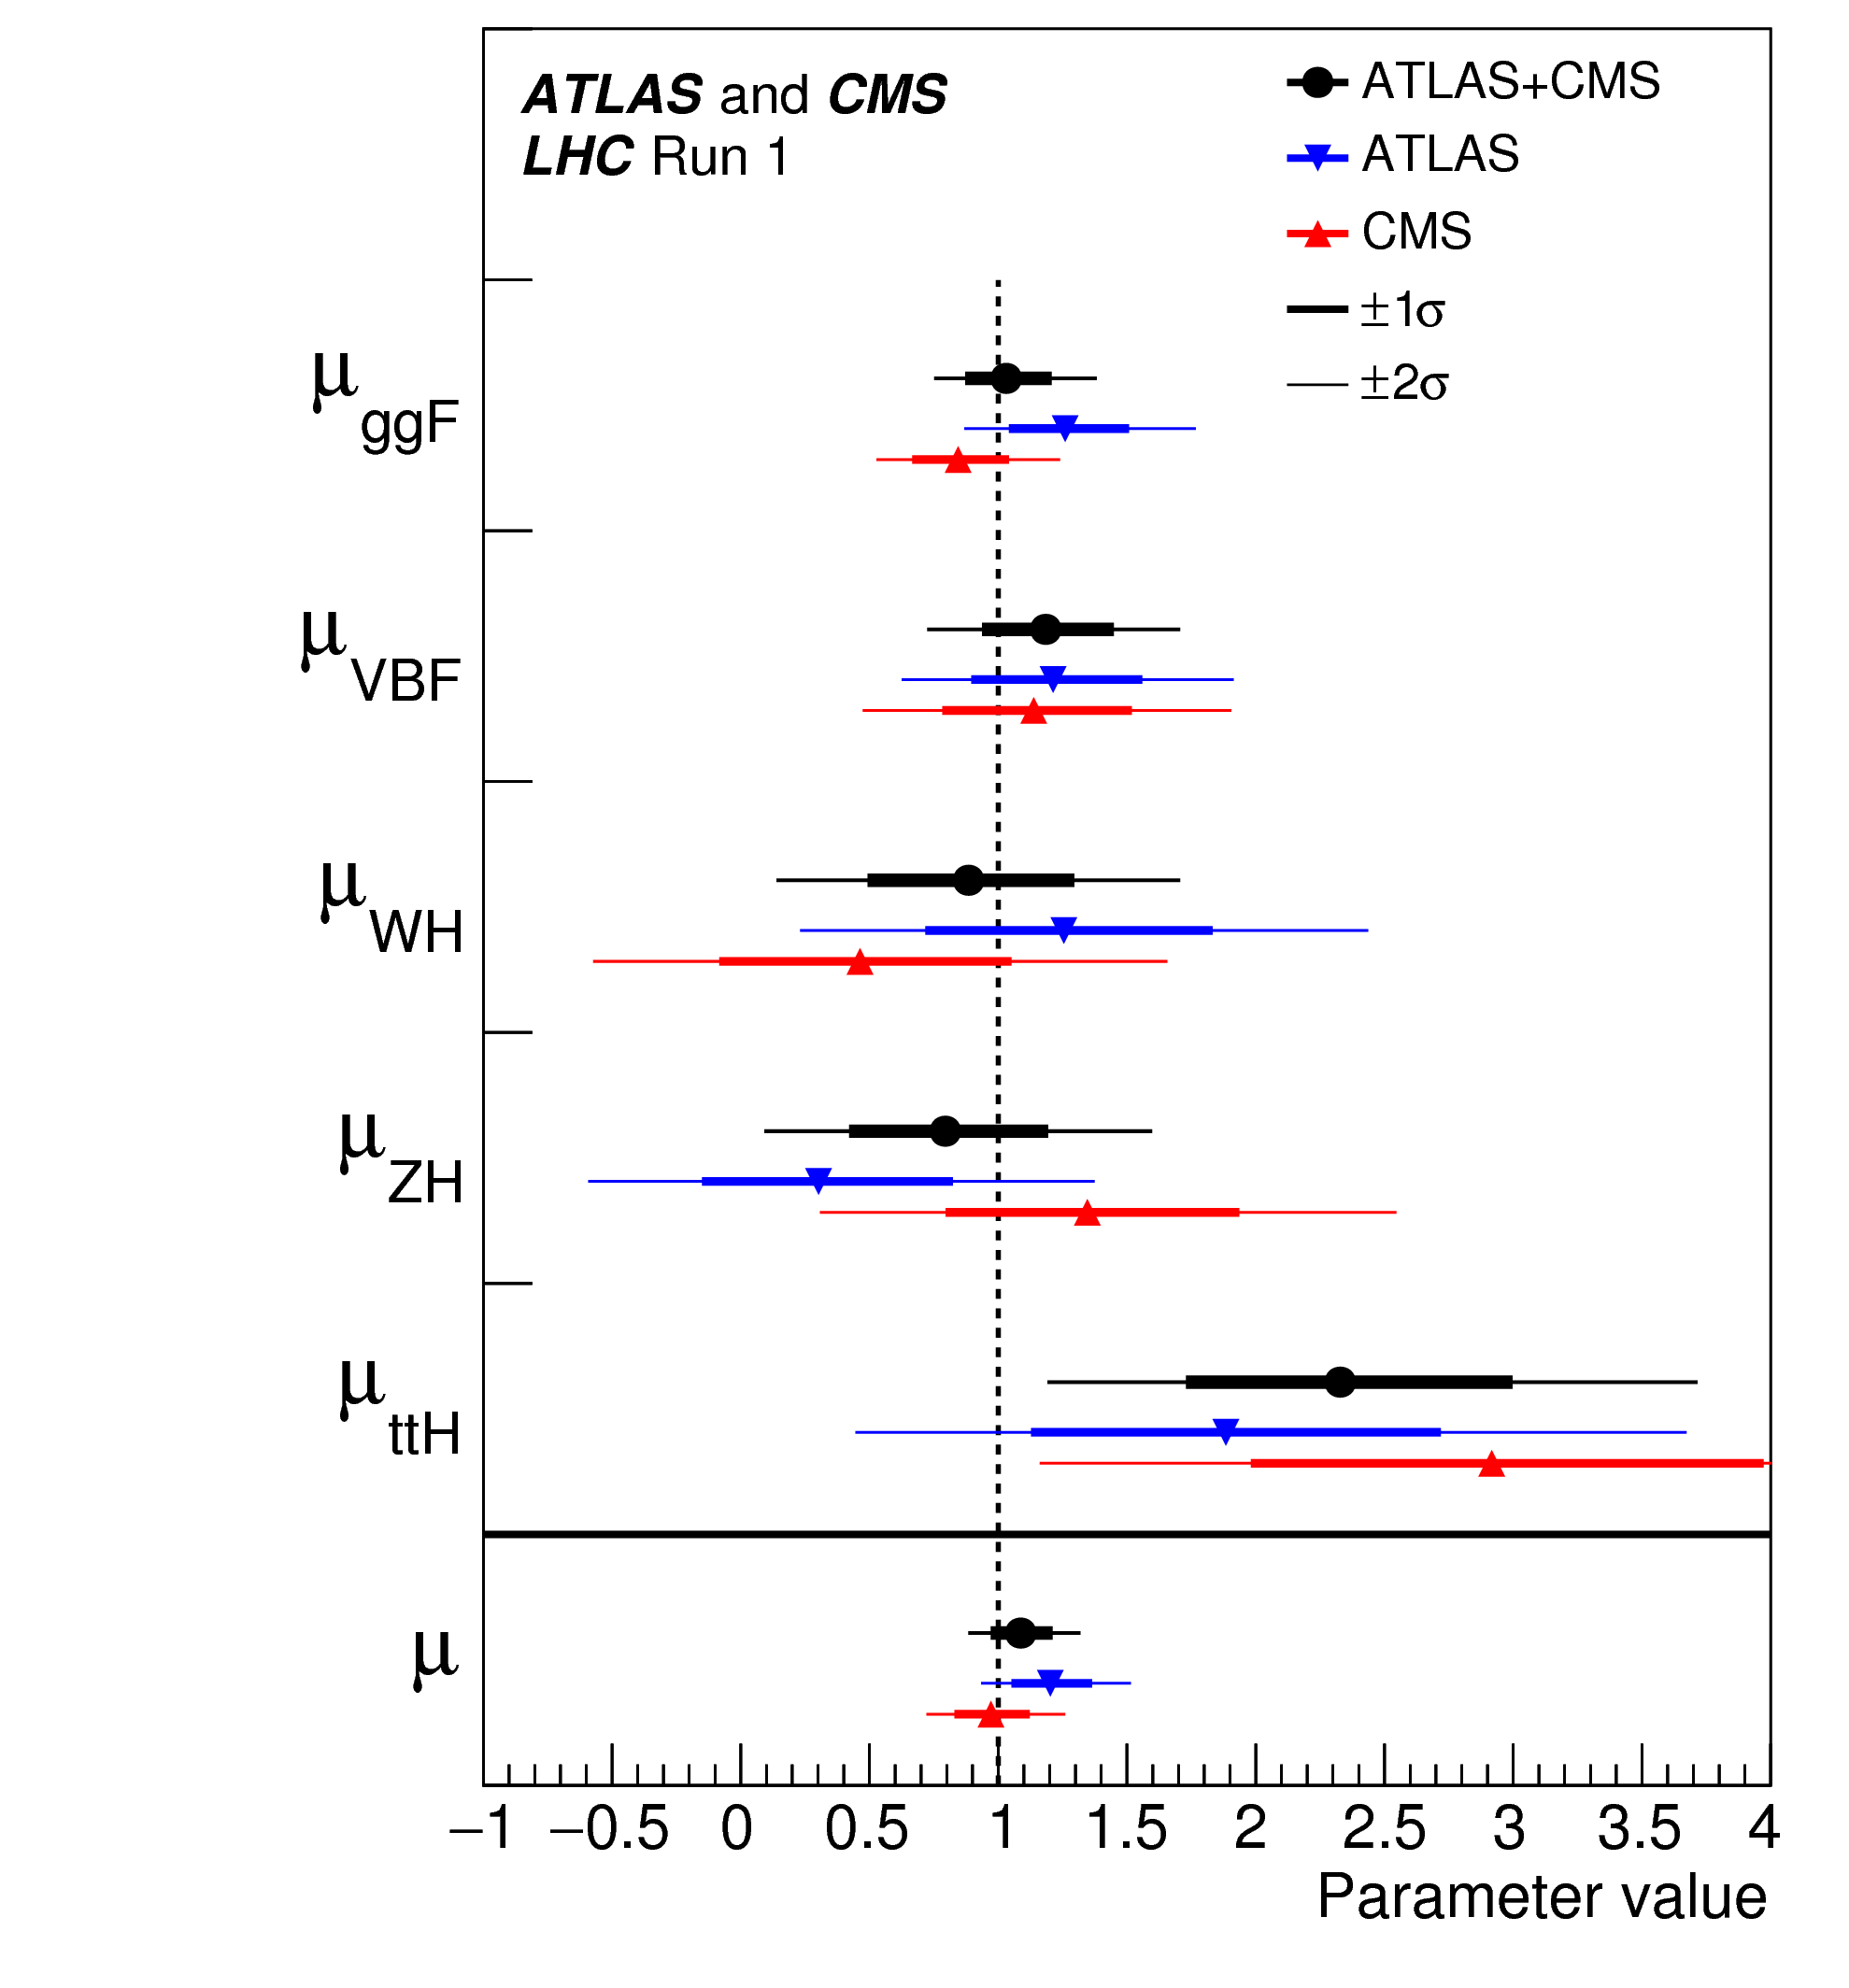
\includegraphics[width=\textwidth]{./figures/theory/signal_strength_production.png}
        \caption{Production modes.}
    \end{subfigure}
    \begin{subfigure}[c]{0.45\textwidth}
        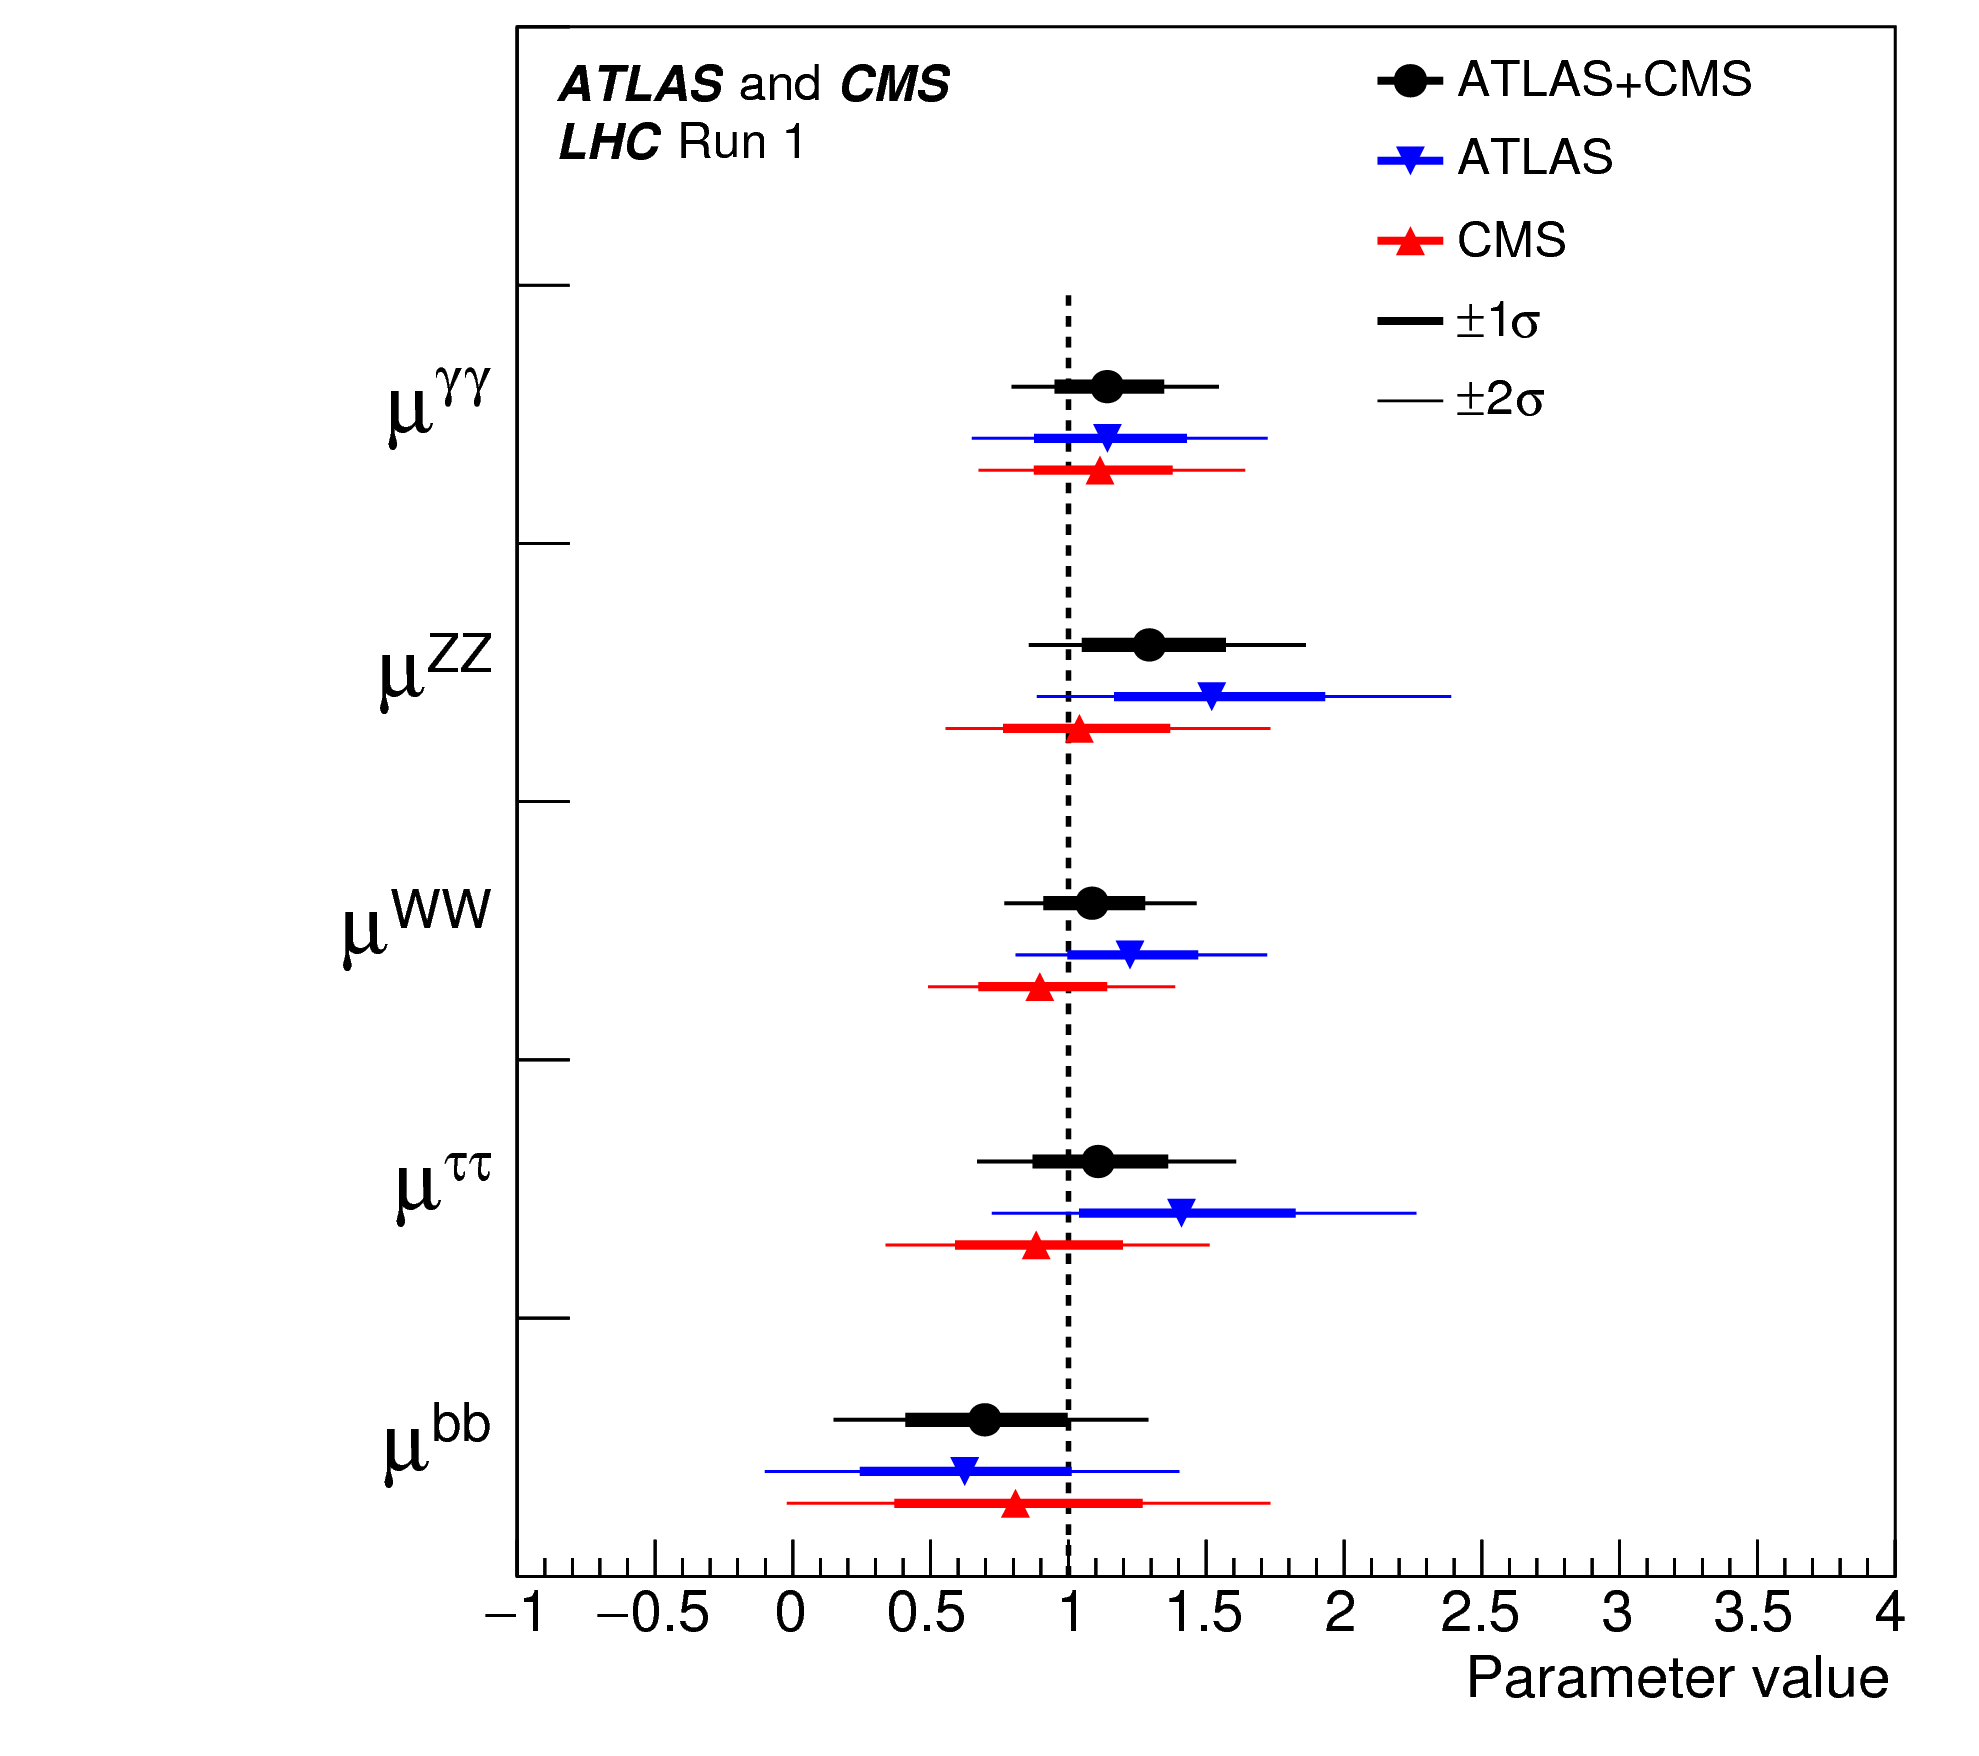
\includegraphics[width=\textwidth]{./figures/theory/signal_strength_decay.png}
        \caption{Decay channels}
    \end{subfigure}
    \caption{Values of the signal strength of the Higgs boson in different production modes (a) and decay channels (b)
             obtained in a combined measurement of the ATLAS and CMS collaborations~\cite{HiggsMuCombined}.}\label{fig:theory:meas:run1:mu}
\end{figure}

Additionally, the LO-coupling modifiers
\begin{equation}
    \kappa_i = \frac{g_i}{g_{,\text{SM}}}
\end{equation}
can be measured, where $g_i$ is the measured coupling strength and $g_{i,\text{SM}}$ the prediction of the Standard Model.
Here, the assumption that beyond the Standard-Model contributions are not present in loops and decay needs to be made.
The normalized coupling strengths are shown in \cref{fig:theory:meas:run1:kappanorm}.
All values are in agreement with the SM expectation of $\kappa_i = 1$.

Furthermore, the reduced coupling strengths $\kappa_F \frac{m_F}{v}$ for fermions and $\sqrt{\kappa_V} \frac{m_V}{v}$ for gauge bosons
can be calculated.
The vacuum expectation value is denoted by $v$.
If all the reduced coupling strengths are depicted as a function of the particle mass, a linear dependence is predicted by the Standard Model.
All values agree within uncertainties with the SM expectation, as can be seen  in \cref{fig:theory:meas:run1:kappareduced}~\

\begin{figure}[htb]
    \centering
    \begin{subfigure}[c]{0.45\textwidth}
        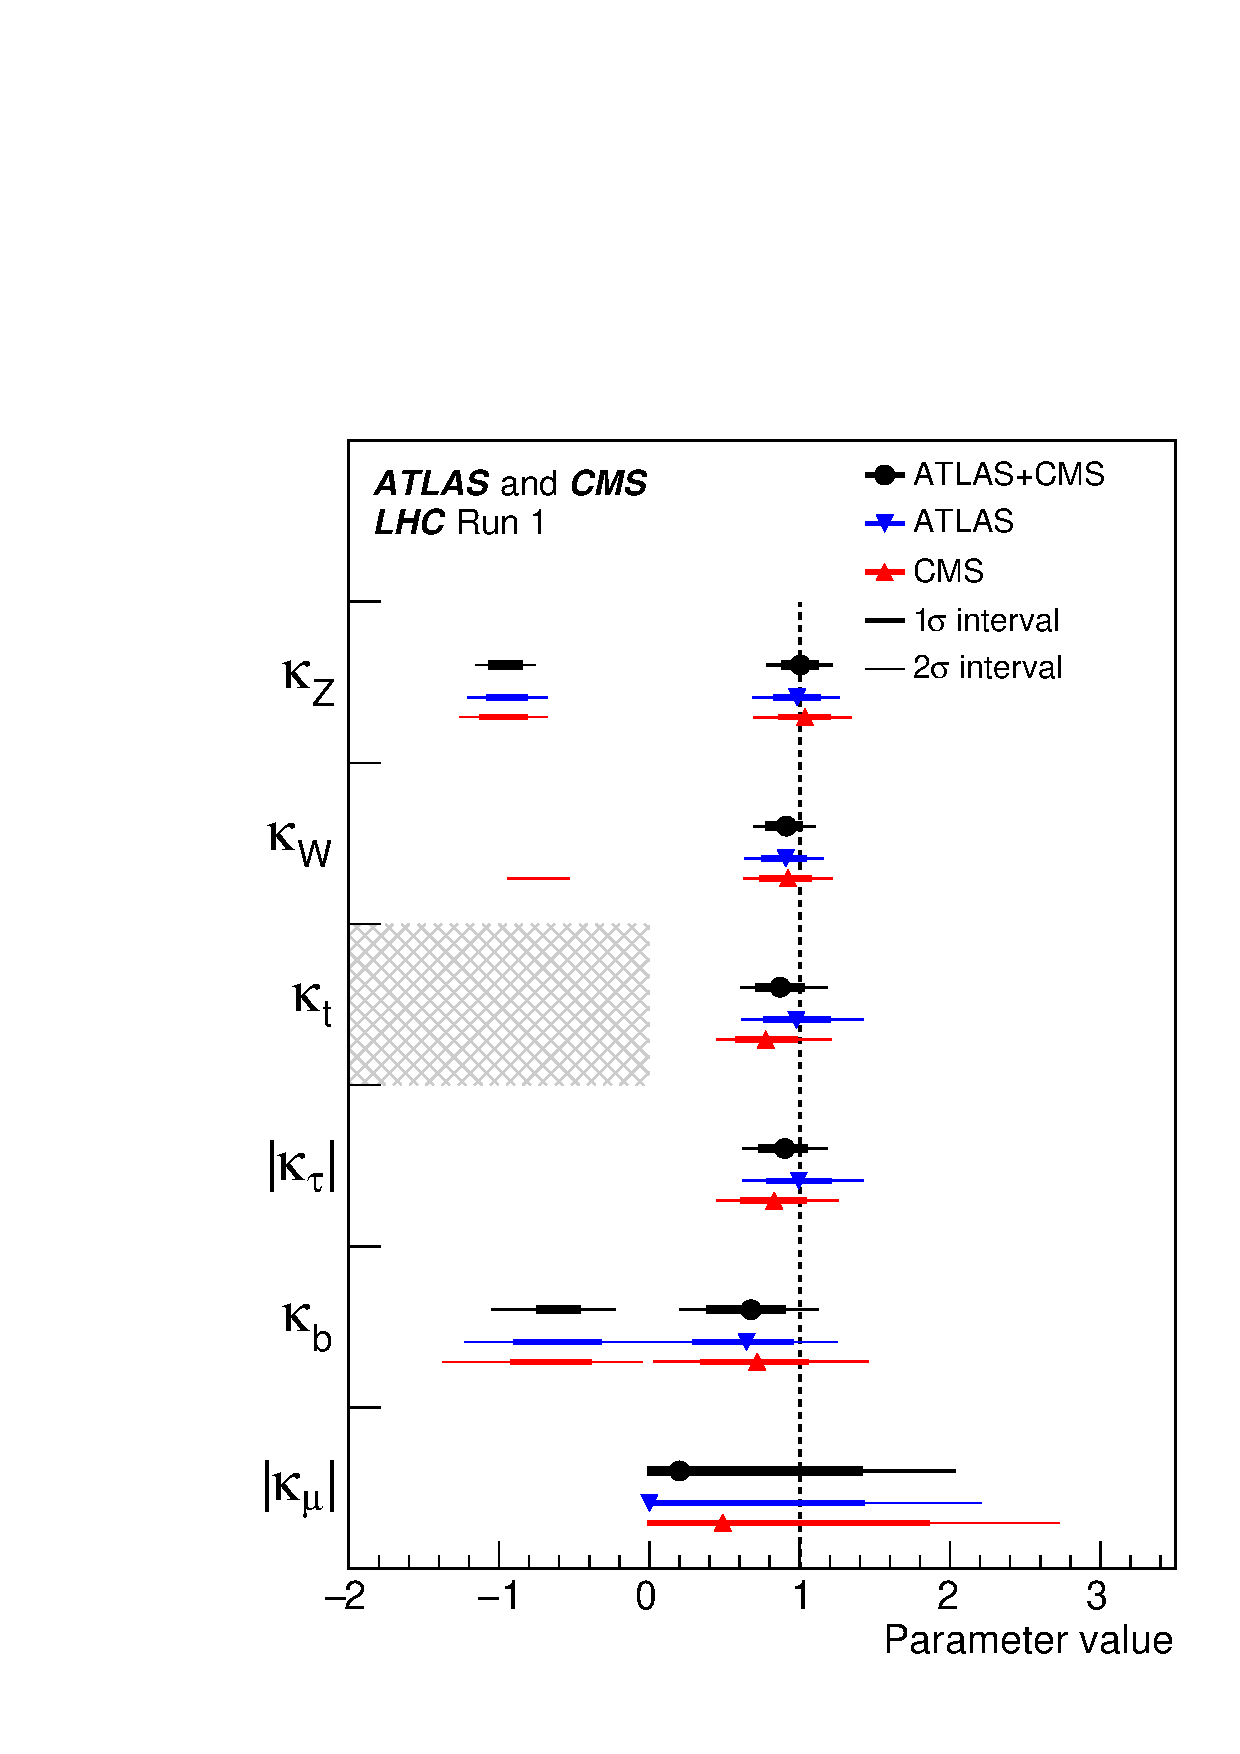
\includegraphics[width=\textwidth]{./figures/theory/coupling_strength.pdf}
        \caption{LO-coupling modifiers}\label{fig:theory:meas:run1:kappanorm}
    \end{subfigure}
    \begin{subfigure}[c]{0.45\textwidth}
        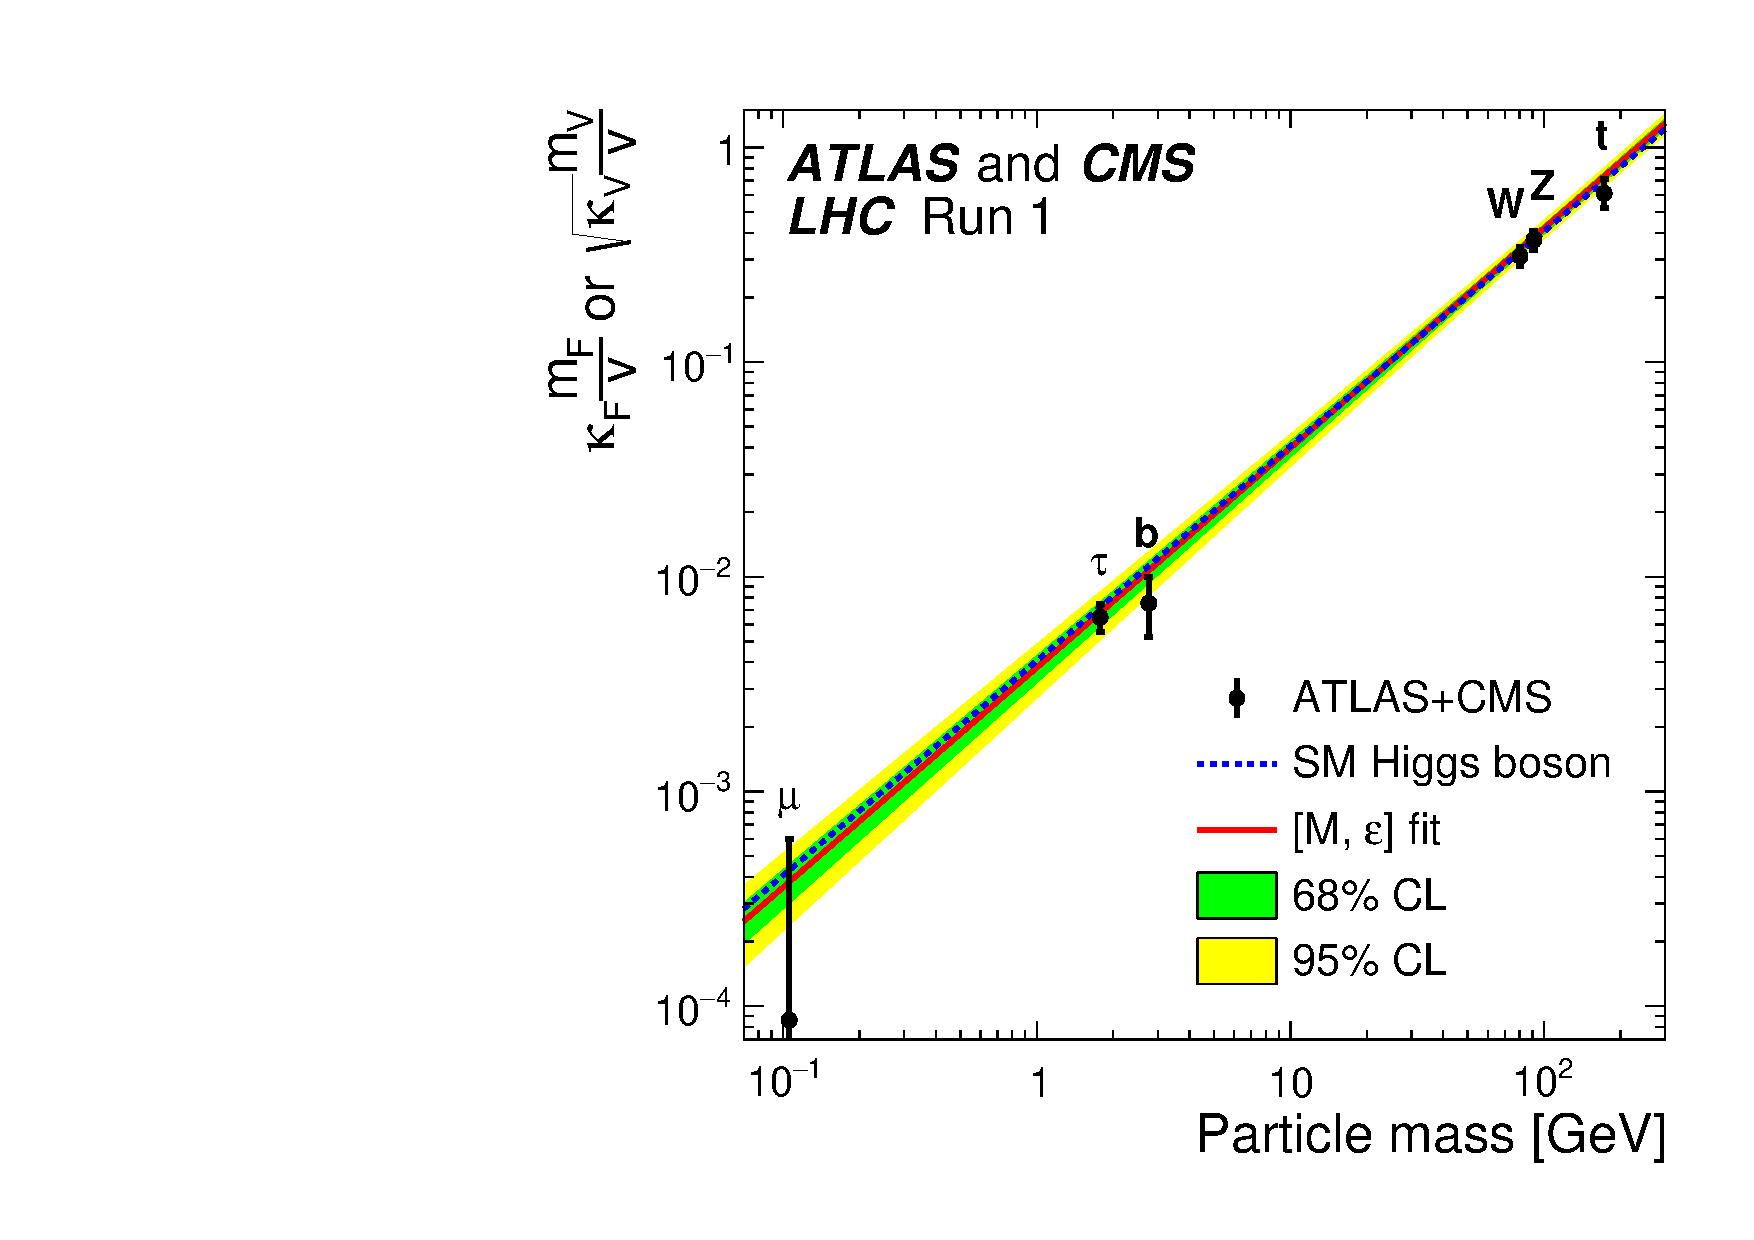
\includegraphics[width=\textwidth]{./figures/theory/reduced_coupling_strength.pdf}
        \caption{Reduced coupling strength}\label{fig:theory:meas:run1:kappareduced}
    \end{subfigure}
    \caption{LO-coupling modifiers of the Higgs boson to different particles (a) and reduced coupling strengths of
             the Higgs boson to different particles as the function of the particle mass (b) determined in a combined measurement
             of the ATLAS and CMS collaboration.
             The prediction of the Standard Model is indicated by the dashed line~\cite{HiggsMuCombined}.}
\end{figure}


\subsubsection{Decay width}\label{subsub:theory:meas:run1:width}

The Standard Model prediction for the decay width of a Higgs boson with a mass of \SI{125}{\GeV} is $\Gamma_\text{H} = \SI{4}{\MeV}$~\cite{YR1}.
This makes the direct measurement of the decay width nearly impossible, since the detector resolution for the $H\to\gamma\gamma$ and
$H \to ZZ \to 4\ell$ channels is around three magnitudes large.

A direct measurement of the decay width of the Higgs boson yielded an upper limit of around \SI{1}{\GeV}~\cite{HiggsGammaDirectATLAS,HiggsGammaDirectCMS}.

Refined analysis techniques are needed for a better limit.
One option is to measure the flight distance of the Higgs boson in the detector, from which the lifetime and subsequently the decay width can be calculated.
This was done by the CMS collaboration and resulted in a lower limit of $\Gamma_H > \SI{3.5e-9}{\MeV}$~\cite{HiggsGammaLifetimeCMS}.

Another possibility is to exploit the production of off-shell production $gg \to H \to VV$ channel.
The ratio between the on- and off-shell signal strengths can be used to determine the decay width of the Higgs boson~\cite{HiggsGammaOffshellCMSZZ},
\begin{equation}
    \frac{\mu_\text{off-shell}}{\mu_\text{on-shell}} = \frac{\Gamma_H}{\Gamma_H^\text{Theory}} \,.
\end{equation}
Both the $WW$ and $ZZ$ decay channel can be used.
Here, the assumption is made that the off-shell cross-section does not depend on the partonic center-of-mass energy and that the background prediction
is not modified by new physics.
The combined limit of those two channels from the CMS collaboration is $\Gamma_H < \SI{13}{\MeV}$~\cite{HiggsGammaOffshellCMSZZ,HiggsGammaOffshellCMSWW}
and from the ATLAS collaboration $\Gamma_H < \SI{22.7}{\MeV}$~\cite{HiggsGammaOffshellATLAS} at \SI{95}{\percent} confidence level (CL).

\subsubsection{Spin and CP properties}\label{subsub:theory:meas:run1:cp}

In the Standard Model the spin and CP properties of the Higgs boson are predicted to be $J^{CP} = 0^+$, i.e.\ a Higgs boson with spin zero
and CP even nature is expected.

Both ATLAS and CMS could confirm this prediction and exclude models with other values of $J^{CP}$ at more than \SI{99.9}{\percent} CL
in measurements using the $H \to \gamma\gamma$ and $H\to ZZ \to 4\ell$ and $H \to WW \to 2\ell2\nu$ decay channels~\cite{HiggsCPATLAS,HiggsCPCMS}.
Especially the CMS collaboration tested a multitude of alternative spin-2 models, as shown in \cref{fig:theory:meas:run1:cp}.

\begin{figure}[htbp]
    \centering
    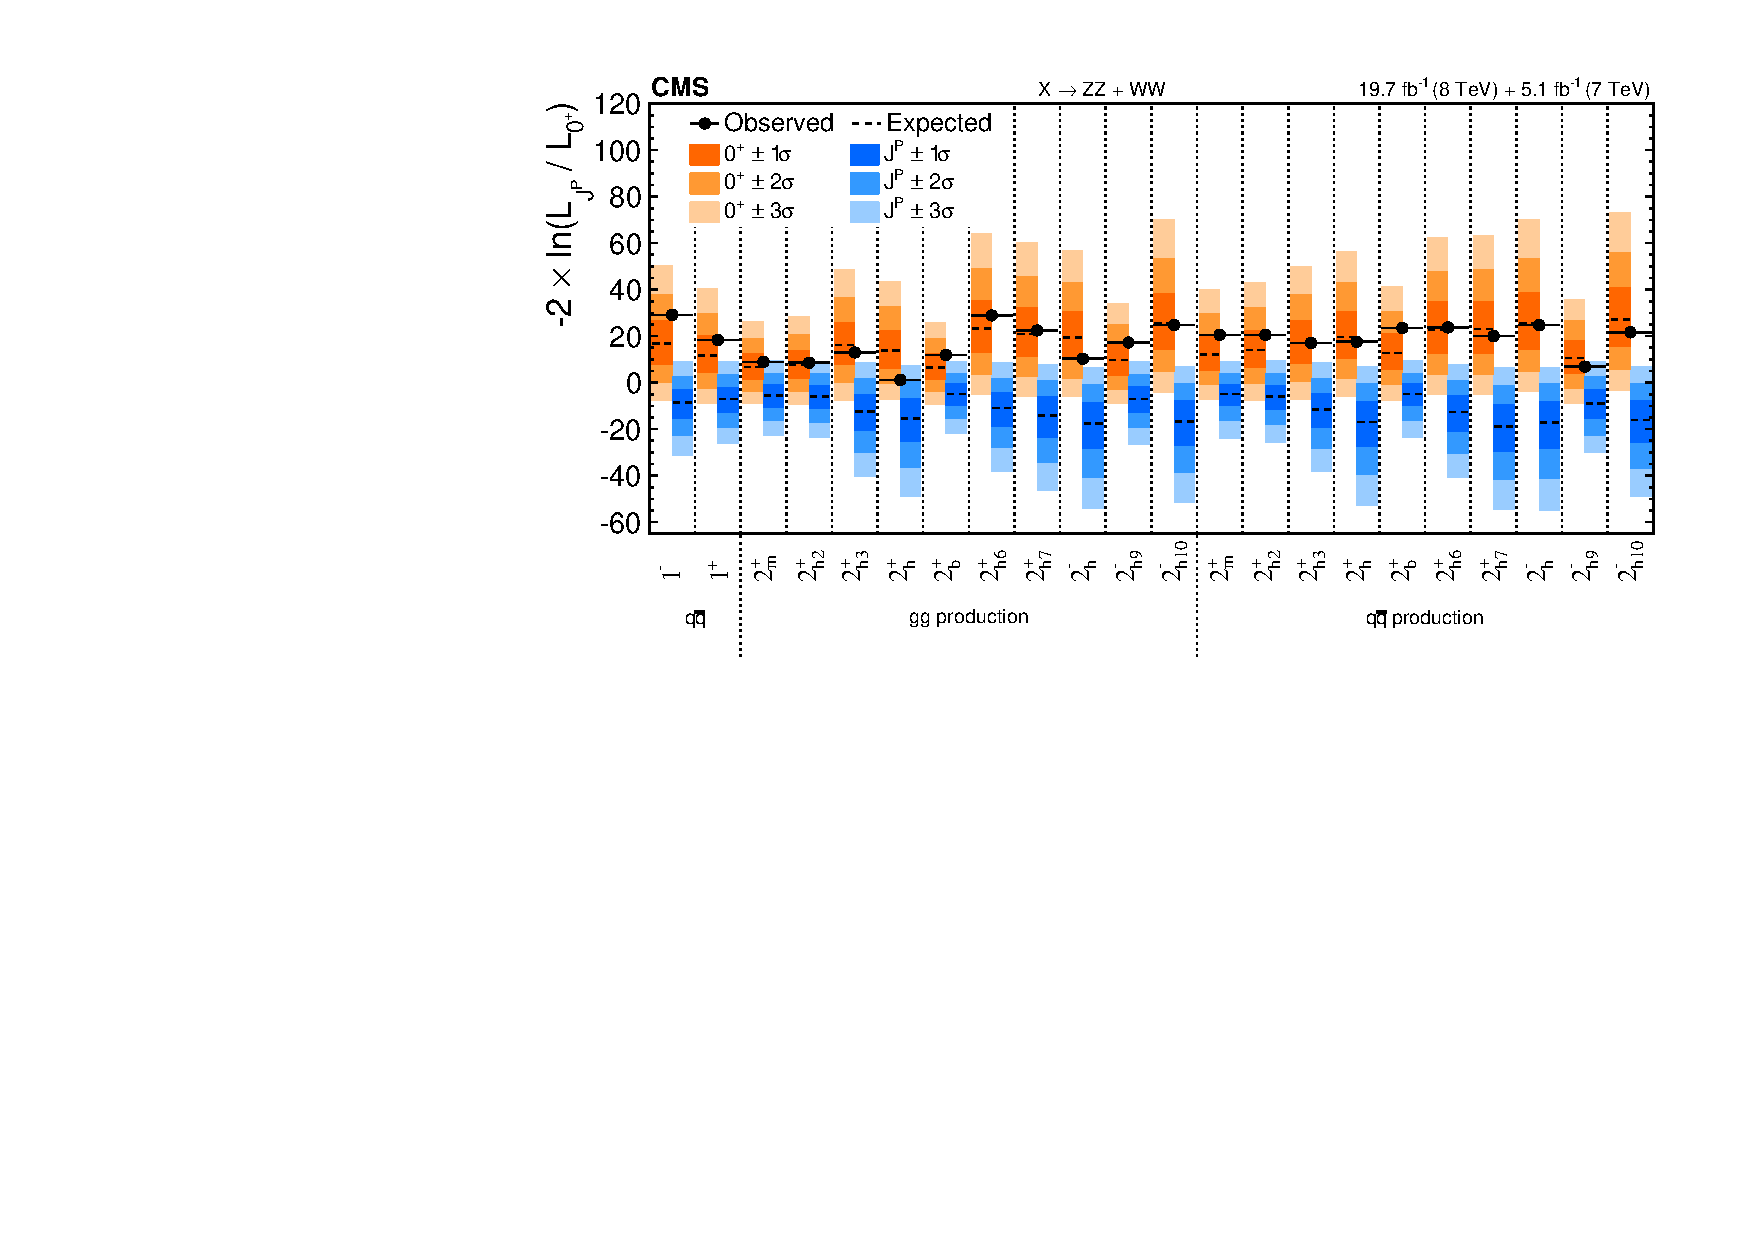
\includegraphics[width=0.9\textwidth]{./figures/theory/cp_cms_results.pdf}
    \caption{Observed and expected values of the test statistic discriminating between the SM
             prediction and other hypothesis from the spin and parity analysis of the CMS
             collaboration~\cite{HiggsCPCMS}.}\label{fig:theory:meas:run1:cp}
\end{figure}

Those measurements do not give information about the sign of the CP operator.
The state $J^{CP} = 1^+$ only indicates that the Higgs boson is invariant under CP transformations.
However, this does not fix the value of the eigenstate of the CP operator.
The possibilities are either $+1$ or $-1$, which are also called CP even or CP odd, respectively, or a mixing between those states.

The mixing between CP-even and CP-odd eigenstates can be measured using the so-called \emph{Optimal Observable}, which
was already used during Run-1 in the $H \to \tau\tau$ decay channel analysis~\cite{HiggsCPTauTau}.
Here, the CP-mixing parameter $\tilde{d}$ provided by the Optimal Observable is directly related to the CP-even nature of the Higgs boson in the
VBF production mode.
A CP-even Higgs-boson results in $\tilde{d} = 0$ while deviations from zero of the CP-mixing parameter would indicate a CP-violating nature of the Higgs boson.

The results of the measurements in~\cite{HiggsCPTauTau} are in agreement with the SM prediction of $\tilde{d} = 0$ and exclude values of $\tilde{d}$ outside of
$\left[-0.11, 0.05\right]$ at a confidence level of \SI{68}{\percent}, as can be seen in \cref{fig:theory:meas:run1:oo}.

Additionally, the CP mixing nature of the Higgs boson can also be measured in the $H \to WW$ and $H \to ZZ$ decay modes~\cite{CPBosonATLAS,CPBosonCMS}.

\begin{figure}[htbp]
    \centering
    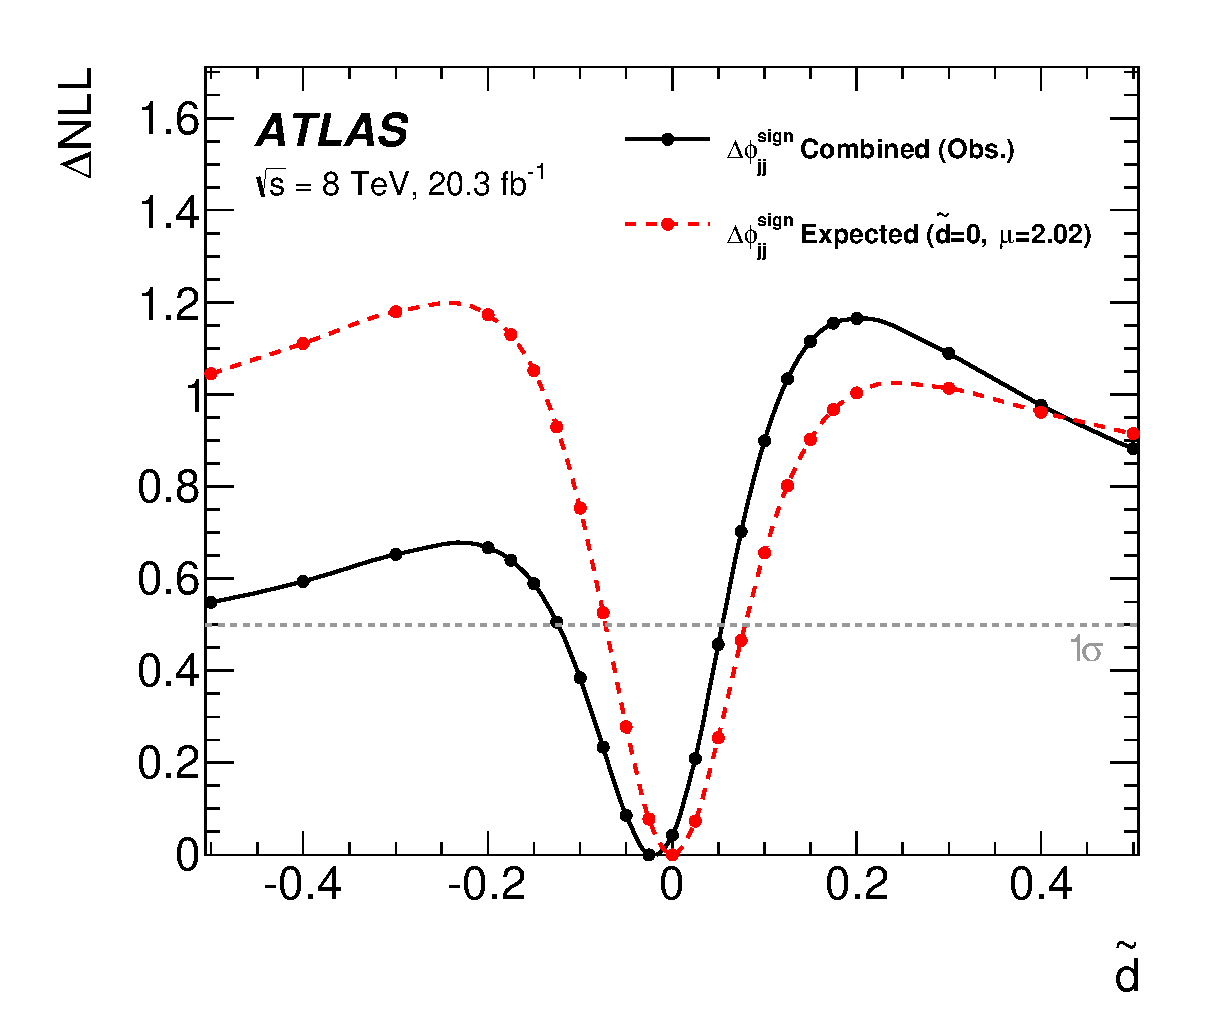
\includegraphics[width=0.5\textwidth]{./figures/theory/cpeven_dtilde.eps}
    \caption{The negative log likelihood ($\Delta \text{NNL}$) as a function of the CP-mixing parameter $\tilde{d}$
             obtained by the Optimal Observable method in the VBF $H\to\tau\tau$ decay channel during Run-1 with the ATLAS detector.
             The minimum of the $\Delta \text{NNL}$ curve corresponds to the best fit value.
             The \SI{68}{\percent} confidence level is indicated by the gray dashed line~\cite{HiggsCPTauTau}.}\label{fig:theory:meas:run1:oo}
\end{figure}

\FloatBarrier{}

\subsection{Measurements during Run-2}\label{sub:theory:meas:run2}

In 2015 the second data-taking period, Run-2, started with an increased center-of-mass energy of \SI{13}{\TeV}.
In the following a few results from the ATLAS experiment using the 2015 and 2016 dataset are presented.

\subsubsection{Total cross section}\label{subsub:theory:meas:run2:totalxsec}

Due to the changing center-of-mass energy the dependence of the total cross section on $\sqrt{s}$ can be investigated.
For this the $H\to\gamma\gamma$ and $H \to ZZ \to 4\ell$ decay channels are used.
The cross section is measured for a center-of-mass energy of $7$ (2011), $8$ (2012), and \SI{13}{\TeV} (2015+2016),
with a dataset corresponding to $4.5$, $20.3$, and $\SI{36.1}{\invfb}$, respectively~\cite{ATLAS-CONF-2017-047}.
The results are shown in \cref{fig:theory:meas:run2:totalxsec}.
Due to the increased cross-section from Run-1 to Run-2, the total cross section is increased by a factor of approximately 2,
agreeing with the SM prediction.

\begin{figure}[htb]
    \centering
    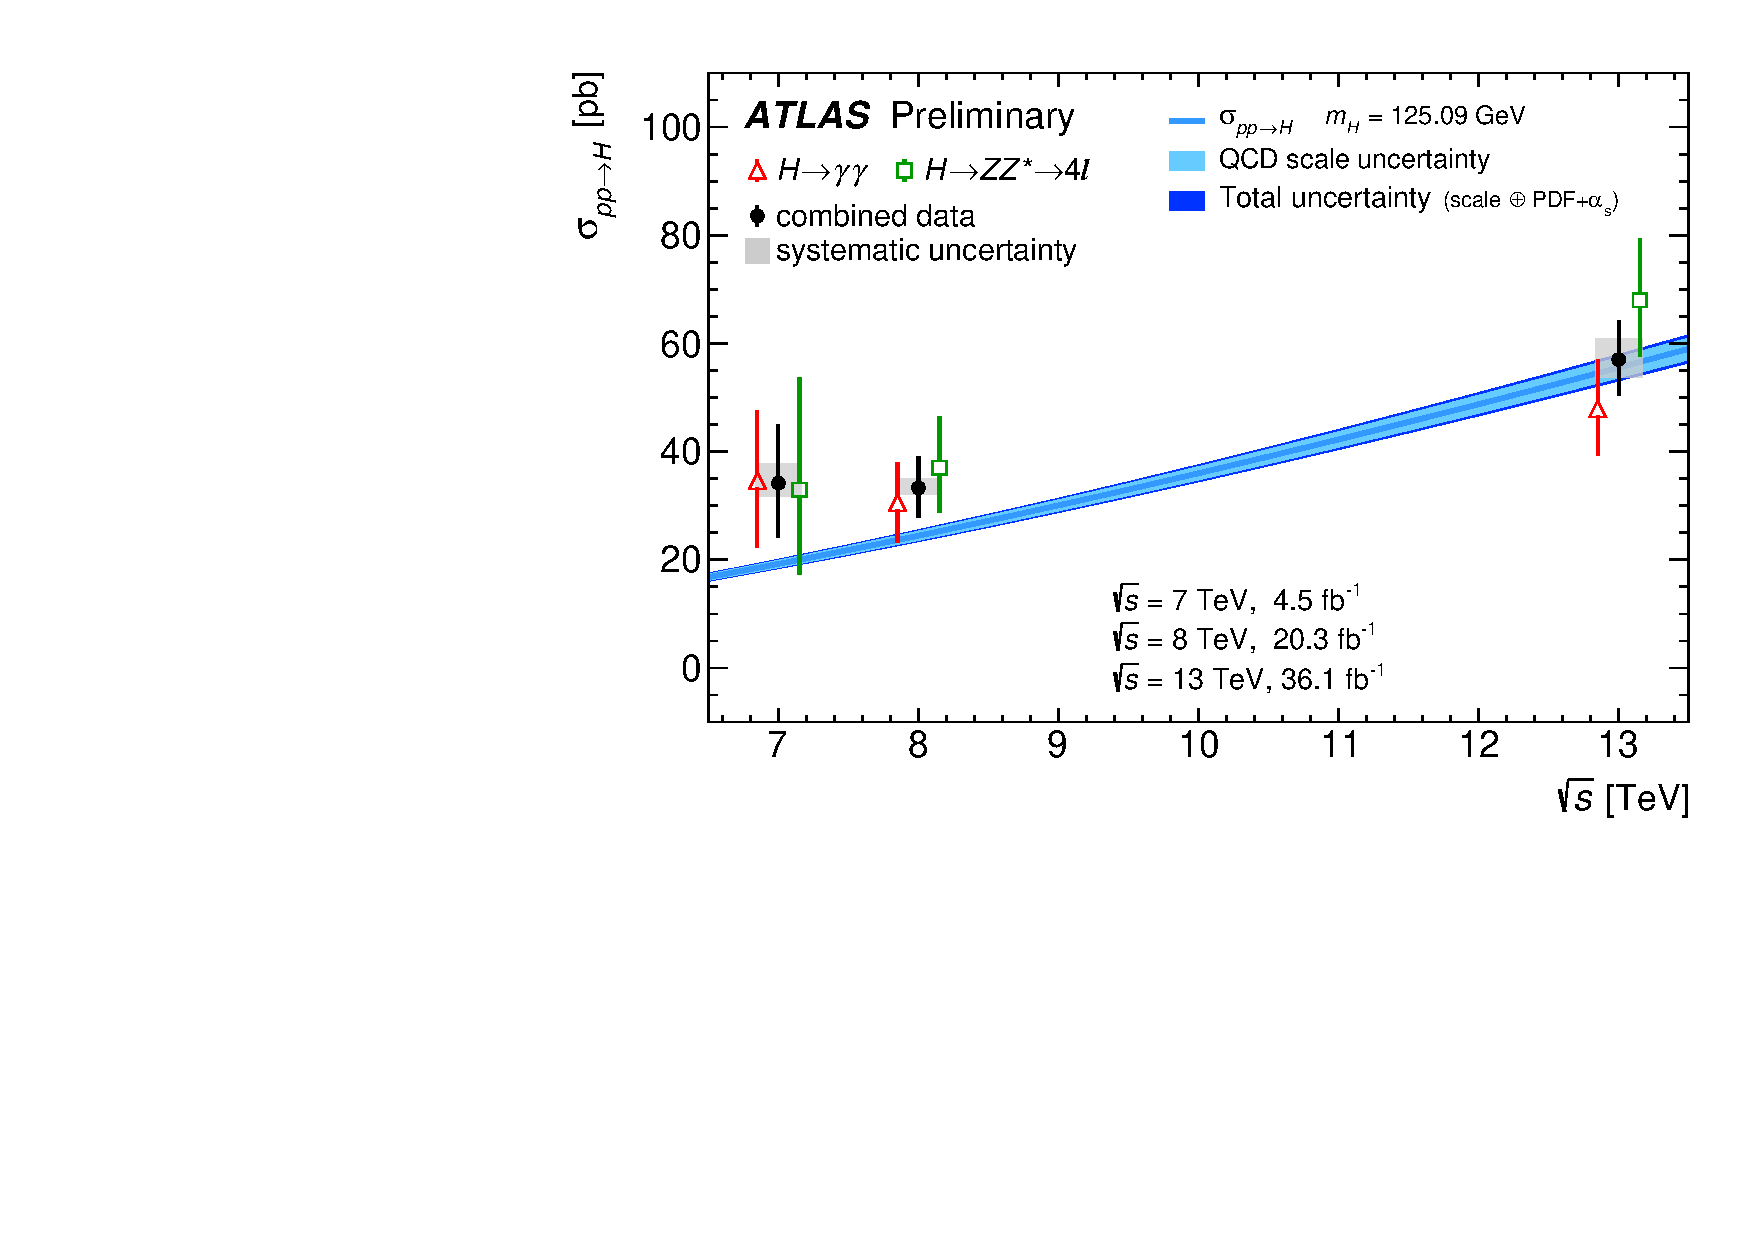
\includegraphics[width=0.9\textwidth]{./figures/theory/total_xsec_run2.pdf}
    \caption{Measurement of the total cross section as a function of the center-of-mass energy in the $H \to \gamma\gamma$
             and $H \to ZZ \to 4\ell$ decay channels with the ATLAS detector~\cite{ATLAS-CONF-2017-047}.}\label{fig:theory:meas:run2:totalxsec}
\end{figure}

\subsubsection{Signal strength}\label{subsub:theory:meas:run2:mu}

The signal strength was measured again with the 2015 and 2016 dataset from Run-2 corresponding to $\SI{36.1}{\invfb}$ with the ATLAS detector.
In the measurement the $H\to\gamma\gamma$ and $H \to ZZ \to 4\ell$ decay channels were used,
yielding a combined signal strength of~\cite{ATLAS-CONF-2017-047}
\begin{equation}
    \mu = 1.09 \pm 0.09 \text{(stat.)} \errud{0.06}{0.05} \text{(exp.)} \errud{0.06}{0.05} \text{(theo.)} \,.
\end{equation}
This is in agreement with the prediction of the Standard Model and previous measurements.

\subsubsection{Mass measurement}\label{subsub:theory:meas:run2:mass}

The mass of the Higgs boson was also determined again using the $H\to\gamma\gamma$ and $H \to ZZ \to 4\ell$ decay channels.
In the measurement the full 2015 and 2016 dataset corresponding to $\SI{36.1}{\invfb}$ is used.
The result is~\cite{ATLAS-CONF-2017-046}
\begin{equation}
    m_H = (124.98 \pm 0.19 \text{(stat.)} + 0.21 \text{(sys.)}) \,, \text{GeV} \,,
\end{equation}
which is in agreement of the combined measurement of Run-1.
